% Appendix

\chapter{} \label{appendix:A}
This appendix section provides supplementary information to Chapter \ref{ch:2}, and is taken directly from the published supplementary materials of \citet{tankersleybasement2022}.

\section{Introduction}
This supplement provides additional information on the assumptions behind the process of determining basement depth from magnetic anomalies (Section \ref{appA:text_S1}), the collection and processing of aeromagnetic line data (Section \ref{appA:text_S2}), the methodology of tying ROSETTA-Ice magnetic basement to ANTOSTRAT acoustic basement \citep{brancolinidescriptive1995}, through the use of Operation IceBridge (OIB) magnetic data \citep{cochranicebridge2014} (Section \ref{appA:text_S3} \& \ref{appA:text_S4}), the gridding, merging, and filtering of the resulting basement grid (Section \ref{appA:text_S5}), the calculation of sediment thickness and $\beta$-factors for the region (Section \ref{appA:text_S6}), and our quantification of uncertainties and comparison with points of previously measured sediment thickness (Section \ref{appA:text_S7}). Sediment thickness comparisons with past seismic surveys are included in Table S1. Also included are supplementary figures showing various additional Ross Ice Shelf grids (Figure \ref{fig:appA_S1}), the Werner deconvolution solutions of OIB flight 403.3 (\ref{fig:appA_S2}), several selected ROSETTA-Ice flight lines with Werner deconvolution solutions (\ref{fig:appA_S3}), unfiltered basement solutions with flight line locations and individual Werner deconvolution solutions (\ref{fig:appA_S4}), uncertainties applied to basement and sediment thickness results (\ref{fig:appA_S5}), and misfit distributions between OIB, ANTOSTRAT, and ROSETTA basement models (\ref{fig:appA_S6}). Python code, within a Jupyter notebook, documents our workflow and figure creation and is accessible here: \url{https://zenodo.org/badge/latestdoi/470814953} or at the GitHub repository: \url{https://github.com/mdtanker/RIS_basement_sediment}. Results in the form of netCDF’s and csv’s are available at \url{https://doi.pangaea.de/10.1594/PANGAEA.941238}, including figures of all ROSETTA-ice flight line basement solutions.

\section{Depth to basement assumptions} \label{appA:text_S1}
Our resulting basement grid is the depth to the shallowest magnetic signal. It is assumed that the crystalline basement in this region produces significantly larger magnetic anomalies compared to the overlying sediment fill. Note that in some instances, such as igneous bodies intruded into sedimentary basin fill, Werner determined solutions fall upon the crest of the intrusion, and the actual top of the crystalline basement could be at a deeper level. Intrusions of small lateral extent will have small widths, resulting in small values of parameter S (susceptibility $\times$ width) and therefore will be removed by our filter (Section \ref{appA:text_S3}). For larger intrusions into existing basins, (i.e. Ross Island and Minna Bluff \cite{coxcontinentwide2023}), the modelled magnetic basement surface will be shallower than the bottom of the sedimentary basin. While this underestimates sediment volume, it better characterizes the competency of the substrate from an ice dynamics perspective. This is similar to how extensive intrusions into basins would be imaged by seismic surveys as shallow basement. However, these extensive regions of late-Cretaceous-Cenozoic magmatism are not expected to be prevalent under the RIS \citep{andrewsresolving2021}.

\section{Magnetic data collection, processing, and Werner deconvolution} \label{appA:text_S2}
Both ROSETTA-Ice and OIB data sets were collected with a Scintrex CS3 Cesium magnetometer. Average flight speeds were 123 m/s and 93 m/s for OIB and ROSETTA-Ice respectively. Altitudes for the sections of OIB flight 403 used here average around 400 m above sea level, while ROSETTA-Ice altitude averaged at 750 m above the ice sheet surface. OIB data were resampled from 20 Hz to 1 Hz to match the frequency of the ROSETTA-Ice data. Both datasets have been despiked, diurnally corrected, and had the International Geomagnetic Reference Field model removed. See \citet{tintoross2019} for more details of the ROSETTA-Ice survey and flight line locations. Due to variable flight elevations, both between and within the datasets, all magnetic data were upward continued to 1000 m above sea level. To avoid artifacts of downwards continuing, any data with flight elevations above 1000 m were removed ($\sim10$\% of the data).\\

Here we use 2D Werner deconvolution \citet{wernerinterpretation1953}, applied to aeromagnetic line data, to image the shallowest magnetic signals in the crust. Assuming that the overlying sediments produce smaller magnetic anomalies than the crystalline basement, we treat the resulting solutions as a depth to the magnetic basement. During Werner deconvolution, moving and expanding windows are passed over the magnetic anomaly line data. Within each window, after linearly detrending the data, the source parameters of the anomalies are estimated with a least-squares approach, assuming the source bodies are infinite-depth dikes or contacts. The source parameters include position (distance along profile and depth), magnetic susceptibility, and source geometry (contact or dike). Solutions are considered valid between 1200 m and 20 km of upward continued flight elevation (approx. 200 m - 19 km bsl). Windows ranged from 500 m - 50 km, with a window shift increment of 1 km and an expansion of 1 km.\\

Due to passing over the data many times with varying window widths, Werner deconvolution produces a depth-scatter of solutions, which tend to cluster vertically beneath the true magnetic sources. Each of these solutions consists of location, depth, susceptibility (S), window width (W), and a simplified source geometry (dike or contact). For contact-type solutions, parameter S is the estimated magnetic susceptibility of the body, while for dike-type solutions, S is the product of susceptibility and dike width. During filtering (Sections \ref{appA:text_S3} \& \ref{appA:text_S4}), a cut-off based on parameter S is used to remove shallow solutions. Since the value of parameter S for contact solutions are typically much smaller than for dike solutions (since they are not multiplied by dike width), only dike solutions have been considered here. To achieve a basement surface from this resulting depth-scatter of solutions, we have utilized parameter-based filtering and clustering, described in Sections \ref{appA:text_S3} \& \ref{appA:text_S4}. This Werner deconvolution process was the same for both OIB and ROSETTA-Ice magnetics data. Werner deconvolution was performed in Geosoft’s Oasis Montaj and subsequent processing of these results was performed in Python, and is included in a Jupyter notebook; \url{https://zenodo.org/badge/latestdoi/470814953}.\\

This magnetic basement approach has been used to map sedimentary basins throughout Antarctica, including the Ross Sea \citep{karnergravity2005}, western Marie Byrd Land \citep{bellidentifying2006}, and Wilkes Subglacial Basin \citep{studingersubice2004, frederickdistribution2016}. Our approach is similar to past studies, but our proximity to well-constrained offshore seismic basement depths \citep{brancolinidescriptive1995} allows us to develop the method further. Most studies display their results as 2D profiles with the depth-scatter of solutions mentioned above, and simply use the tops of the clusters as the basement depth. By comparison with seismic basement, we have developed a reliable, automated method of ‘draping’ a surface over these depth-scattered solutions to produce a 3D surface. This process is described below.

\section{Tying magnetic basement to seismic basement} \label{appA:text_S3}
To validate the method described in Section \ref{appA:text_S2} and address uncertainty we perform Werner deconvolution for OIB magnetics data \citep[Figure \ref{fig:chp2_Bathy_Mag}b,][]{cochranicebridge2014} over the Ross Sea. Here, ice-free conditions have permitted shipborne seismic surveys to image basement depths in the region. These have been compiled by the Antarctic Offshore Acoustic Stratigraphy project (ANTOSTRAT) \citep{brancolinidescriptive1995} (Figure \ref{fig:chp2_Bathy_Mag}b). The basement was not imaged for the deepest portions of the basins and data coverage of actual basement reflectors, versus interpolation between basement reflectors, is not reported. Werner deconvolution (Section \ref{appA:text_S2}) produces a series of many solutions (black dots in Figures \ref{fig:chp2_OIB_403_1} \& \ref{fig:appA_S2}) at each window along the line.\\

To achieve a basement surface, instead of a depth-scatter of solutions, solutions were filtered based on Werner window width (W) and the product of magnetic susceptibility and body width (parameter S). Filtered solutions (black circles, scaled to parameter S in Figures \ref{fig:chp2_OIB_403_1} \& \ref{fig:appA_S2}) were then horizontally binned with variable bin sizes (parameter B) (vertical grey lines in Figures \ref{fig:chp2_OIB_403_1} \& \ref{fig:appA_S2}). Bins with a minimum count of solutions (parameter C) were retained, and the depth of the bin centre was set to the 95th-percentile depth of the solutions in the bin. This removed spurious shallow solutions, while effectively retaining the ‘top’ of the magnetic signal. These bin centres (orange crosses in Figures \ref{fig:chp2_OIB_403_1} \& \ref{fig:appA_S2}) were then interpolated, producing our model of magnetic basement depths (orange line in Figures \ref{fig:chp2_OIB_403_1} \& \ref{fig:appA_S2}). The above filtering techniques removed the solutions above the basement, and the clustering technique fitted a surface over the remaining points, which represents the top of the basement. This interpolated line allowed a direct comparison between ANTOSTRAT seismic basement and OIB magnetic basement.\\

We varied each of the four parameters (W, S, B, and C) with 21 different values and conducted the above procedures for all unique combinations of them on OIB line 403, segments 1 and 3, in the Ross Sea (location in Figure \ref{fig:chp2_Bathy_Mag}b). This resulted in 194,481 iterations, for each of which we calculated a mean absolute difference at points every 5 km between ANTOSTRAT seismic basement and the resulting OIB magnetic basement. We found the parameter values which produced the closest match between OIB magnetic basement and ANTOSTRAT seismic basement, as shown in Figures \ref{fig:chp2_OIB_403_1} \& \ref{fig:appA_S2}. These resulting values were a maximum Werner deconvolution window width (parameter W) of 10 km, a minimum product of magnetic susceptibility and body width (parameter S) of 1.0, a horizontal bin width (parameter B) of 36 km, and a minimum number of solutions per bin (parameter C) of 6. The median absolute misfit between OIB and ANTOSTRAT basement for the two line-segments was 480 m (260 m for Line 403.1 (Figure \ref{fig:chp2_OIB_403_1}), and 1040 m for Line 403.3 (Figure \ref{fig:appA_S2})). This equates to 11\% of average ANTOSTRAT depths for the two lines. The close fit between the OIB magnetic basement and the ANTOSTRAT seismic basement both supports the validity of this method and gives us the parameters necessary to repeat this method for data over the RIS.

\section{Tying Ross Sea magnetic basement to Ross Ice Shelf magnetic basement} \label{appA:text_S4}
Having optimized our method to match OIB magnetic basement to ANTOSTRAT seismic basement in the Ross Sea (Section \ref{appA:text_S3}, Figures \ref{fig:chp2_OIB_403_1} \& \ref{fig:appA_S2}), we now optimize the method to match ROSETTA-Ice magnetic basement to OIB magnetic basement. This additional optimization is necessary due to differences in processing and survey design, including flight elevations, speed, aircraft, mounting equipment used, and frequency of recording. With the optimized parameters for OIB data (Section \ref{appA:text_S3}), we calculate magnetic basement for OIB flight 404 over the ice shelf. We treat this as the ’true’ basement and update the filtering and clustering parameters (Section \ref{appA:text_S2}) to minimize the misfit between OIB basement and the resulting ROSETTA-Ice basement. This tuning was performed on ROSETTA-Ice lines 590 and 650, which were coincident with segments from OIB line 404 (location in Figures \ref{fig:chp2_Bathy_Mag}b \& \ref{fig:appA_S4}). Optimal parameters to match ROSETTA-Ice solutions to OIB basement are found to be W\textless26 km, S\textgreater1.2, B=36 km, and C\textgreater40, resulting in a median absolute misfit between OIB basement and ROSETTA-Ice solutions of 400 m (630 m for line 404.590 (Figure \ref{fig:appA_S3}e) and 310 m for line 404.590 (Figure \ref{fig:appA_S3}f). This equates to 18\% of OIB depths for the two lines. With these parameters which best match ROSETTA magnetic basement to OIB magnetic basement, we performed the same procedure on all the ROSETTA-ice flight lines. A selection of these lines, and the two ties to OIB 404, are shown in Figure \ref{fig:appA_S3}. All ROSETTA-ice flight line solutions are available as images at the PANGAEA link.

\section{Gridding, merging, and filtering} \label{appA:text_S5}
The above processes were performed on all ROSETTA-ice flight lines (white lines in Figure \ref{fig:appA_S4}), including the N-S tie lines at $\sim55$ km spacing. Where the tie lines crossed over  the E-W flight lines, some resulting basement solutions (black dots in Figure \ref{fig:appA_S4}) are nearby those from the crossing line. Since we are interested in the shallowest magnetic signals, we have retained only the shallowest solution with 8 km cells across our region. Since bin widths (parameter B) were set to 36 km, the nearest solutions along individual lines were further apart than the 8 km cell. The closest spacing of E-W flight lines was 10 km, so this process only affected solutions at the crossover between N-S and E-W lines. These points were then gridded with a 5 km cell size and a minimum curvature spline with a tension factor of 0.35 \cite{smithgridding1990} (Figure \ref{fig:appA_S4}). This grid was then merged with a Ross Sea seismic basement grid. The Ross Sea grid, while mostly ANTOSTRAT data, was sourced from a regional compilation of sediment thicknesses \citep{lindequepreglacial2016, wilsonwest2009} we have subtracted from bathymetry depths \citep{morlighemdeep2020} to achieve basement depths. Where the grids overlap near the ice shelf edge, we retain our RIS values. To aid in the merging at the overlaps, and to match RIS basement wavelengths to the characteristic basement wavelengths of ANTOSTRAT, we filtered the merged grid with an 80 km Gaussian filter (Figure \ref{fig:chp2_Basement_sediment}a). This filtering was performed with a variety of wavelengths (20-120 km), where we found filters \textless 80 km didn’t significantly alter the regional basement, while filters \textgreater 80 km excessively smoothed the basement topography. A few locations with anomalously shallow basement were set equal to BedMachine bathymetry.

\section{Sediment thickness and $\beta$-factor calculations} \label{appA:text_S6}
With the regional basement model (Figure \ref{fig:chp2_Basement_sediment}a) including RIS magnetic basement and offshore seismic basement, we calculated sediment thickness (Figure \ref{fig:chp2_Basement_sediment}b) by subtracting the grid from Bedmachine bathymetry depths \citep[Figure \ref{fig:chp2_Bathy_Mag}a \& \ref{fig:appA_S1}e,][]{morlighemdeep2020}. Previous estimates of sediment thickness for the sub-RIS come from the extrapolation of gravity anomalies with bathymetry trends \citep{wilsonwest2009}. These were included in the \citet{lindequepreglacial2016} compilation (Figure \ref{fig:appA_S1}d). Eocene Oligocene boundary paleotopographic reconstructions \citep{wilsonantarctic2012, paxmanreconstructions2019} assumed this sediment estimate was post-Eocene and used it as their maximum sub-RIS sediment thickness, incorporated into their minimum surface reconstruction. The thickness of sediment affects onshore erosion estimates, surface raising due to deposition, and isostatic surface subsidence to due loading. For their maximum paleotopographic reconstructions, they used a thinner sediment model, with the same general trends \citep{wilsonwest2009}. Figure \ref{fig:appA_S1} (c, d, \& f) shows the comparison between the sediment thickness models. Figure \ref{fig:appA_S1}f colorbar histogram shows the distribution, with our values having a mean thickness $\sim115$ m greater than the past model. Yet, along the Siple Coast, we show much greater discrepancies, up to 2 km thicker. $\beta$-factor, the ratio of initial crustal thickness to final crustal thickness, is useful for quantifying the thinning of crust in extensional settings. We calculate a distribution of $\beta$-factors beneath the RIS by assuming a uniform initial crustal thickness and dividing it by current crustal thickness. We pick an initial crustal thickness of 38 km, which represents a global average for un-thinned plateau-type crust \citep{mooneycrust1998}, and has been used for the West Antarctic Rift System $\beta$-factor calculations \citep{müllereocene2007}. For the final (current) crustal thickness, we use a continent-wide Moho model from surface wave observations to define the bottom of the crust \citep{ansvelocity2015}. For the top of the crust, we use our resulting RIS basement grid.

\section{Uncertainties} \label{appA:text_S7}
We estimated a representative uncertainty for our basement model by examining the misfit of our modelled basement compared to offshore seismic basement depths \citep{brancolinidescriptive1995}. We did this by sampling our OIB magnetic basement estimate and the coincident ANTOSTRAT basement at 1 km intervals along lines 403.1 and 403.3 (Figures \ref{fig:chp2_OIB_403_1} and \ref{fig:appA_S2}) and compared the values. The resulting absolute values of the differences don’t exhibit a normal distribution (Figure \ref{fig:appA_S6}a); therefore, we use the median of the absolute misfit ($\pm480$ m) as the basement model uncertainty. This equates to 22\% of average basement depths for the sub-RIS. We performed a similar analysis between OIB magnetic basement and ROSETTA-Ice magnetic basement for coincident lines 590 and 650 (Figure \ref{fig:appA_S3} e \& f). This resulted in a median absolute misfit of 400 m (Figure \ref{fig:appA_S6}b). \citet{tintoross2019} report an uncertainty of 68 m for their bathymetry model. Incorporating this with our basement model gives an uncertainty of 550 m (37\% of average thickness) for our sediment thickness results. Comparison with sub-RIS sediment thickness and distribution results from a variety of methods, including active source seismic surveys (Table \ref{table:appA_S1} and references within), seismic radial anisotropy \citep{zhouradial2022}, geophysical machine learning \citep{lisedimentary2022}, and magnetotelluric surveying \citep{gustafsondynamic2022}, all show general agreement with our results.


\begin{table}[] 
\resizebox{\textwidth}{!}{%
\begin{tabular}{lllll} 
\textbf{Name} & \textbf{Reference}              & \textbf{\begin{tabular}[c]{@{}l@{}}Seismic sediment \\ thickness (m)\end{tabular}} & \textbf{\begin{tabular}[c]{@{}l@{}}Magnetic sediment \\ thickness (m)\end{tabular}} & \textbf{\begin{tabular}[c]{@{}l@{}}Absolute \\ difference (m)\end{tabular}} \\
CIR           & \citep{rooneyseismic1987}      & 400                                                                                & 514                                                                                 & 114                                                                         \\
I10S          & \citep{robertsonross1989}       & $750\pm100$                                                                        & 1281                                                                                & 818                                                                         \\
J9DC          & \citep{greischaranalysis1992}   & 1350                                                                               & 770                                                                                 & 580                                                                         \\
BC            & \citep{robertsonross1989}       & $1900\pm400$                                                                       & 1082                                                                                & 818                                                                         \\
RI            & \citep{greischaranalysis1992}   & 850                                                                                & 822                                                                                 & 28                                                                          \\
C49           & \citep{crarymarinesediment1961} & 754                                                                                & 1162                                                                                & 408                                                                         \\
LAS           & \citep{crarymarinesediment1961} & 1325                                                                               & 1799                                                                                & 474                                                                         \\
Q13           & \citep{greischaranalysis1992}   & $255\pm145$                                                                        & 721                                                                                 & 466                                                                        
\end{tabular}%
}
\caption[Previous Ross Ice Shelf seismic sediment thickness measurements]{Previous seismic sediment thickness results for the Ross Ice Shelf. Stations names are labelled in Figure \ref{fig:chp2_Basement_sediment}b. Magnetic sediment thickness column shows our sampled results at the location of each station. Comparing the seismic estimates with our sediment thickness at the eight stations gives a median absolute misfit of 470 m.}
\label{table:appA_S1}
\end{table}

\begin{figure}[!ht]
    \centering
    \includegraphics[width=.95\textwidth]{figures/chp2/figure_S1.png}
    \caption[Various Ross Ice Shelf grids]{\textbf{a)} ROSETTA-Ice free air gravity \citep{tintoross2019}. Shaded yellow regions are shallow basement ($<\sim1600$ mbsl), shaded blue regions are deep basement ($>\sim2600$ mbsl). \textbf{b)} ROSETTA-Ice airborne magnetic anomaly data \citep{tintoross2019}. \textbf{c)} Sediment thickness from this study (same as Figure \ref{fig:chp2_Basement_sediment}b), with 1 km contours. \textbf{d)} Sediment thickness from a regional compilation \citep[Section \ref{appA:text_S6},][]{lindequepreglacial2016, wilsonwest2009}, with 1 km contours. \textbf{e)} BedMachine2 bathymetry \citep{morlighemdeep2020}, from which sediment thickness in c) was calculated. \textbf{f)} Difference between c) and d). Red signifies our results have more sediment, while blue signifies our results have less sediment. Histogram shows data distribution, with mean value (black) at 115 m. Inferred faults in a), b), c), and e) same as Figure \ref{fig:chp2_Tectonic_interpretation}a. Grounding line and coastlines in black \citep{rignoticeshelf2013}. Projection is Antarctic Polar Stereographic: EPSG 3031.}
    \label{fig:appA_S1}
\end{figure}

\begin{figure}[!ht]
    \centering
    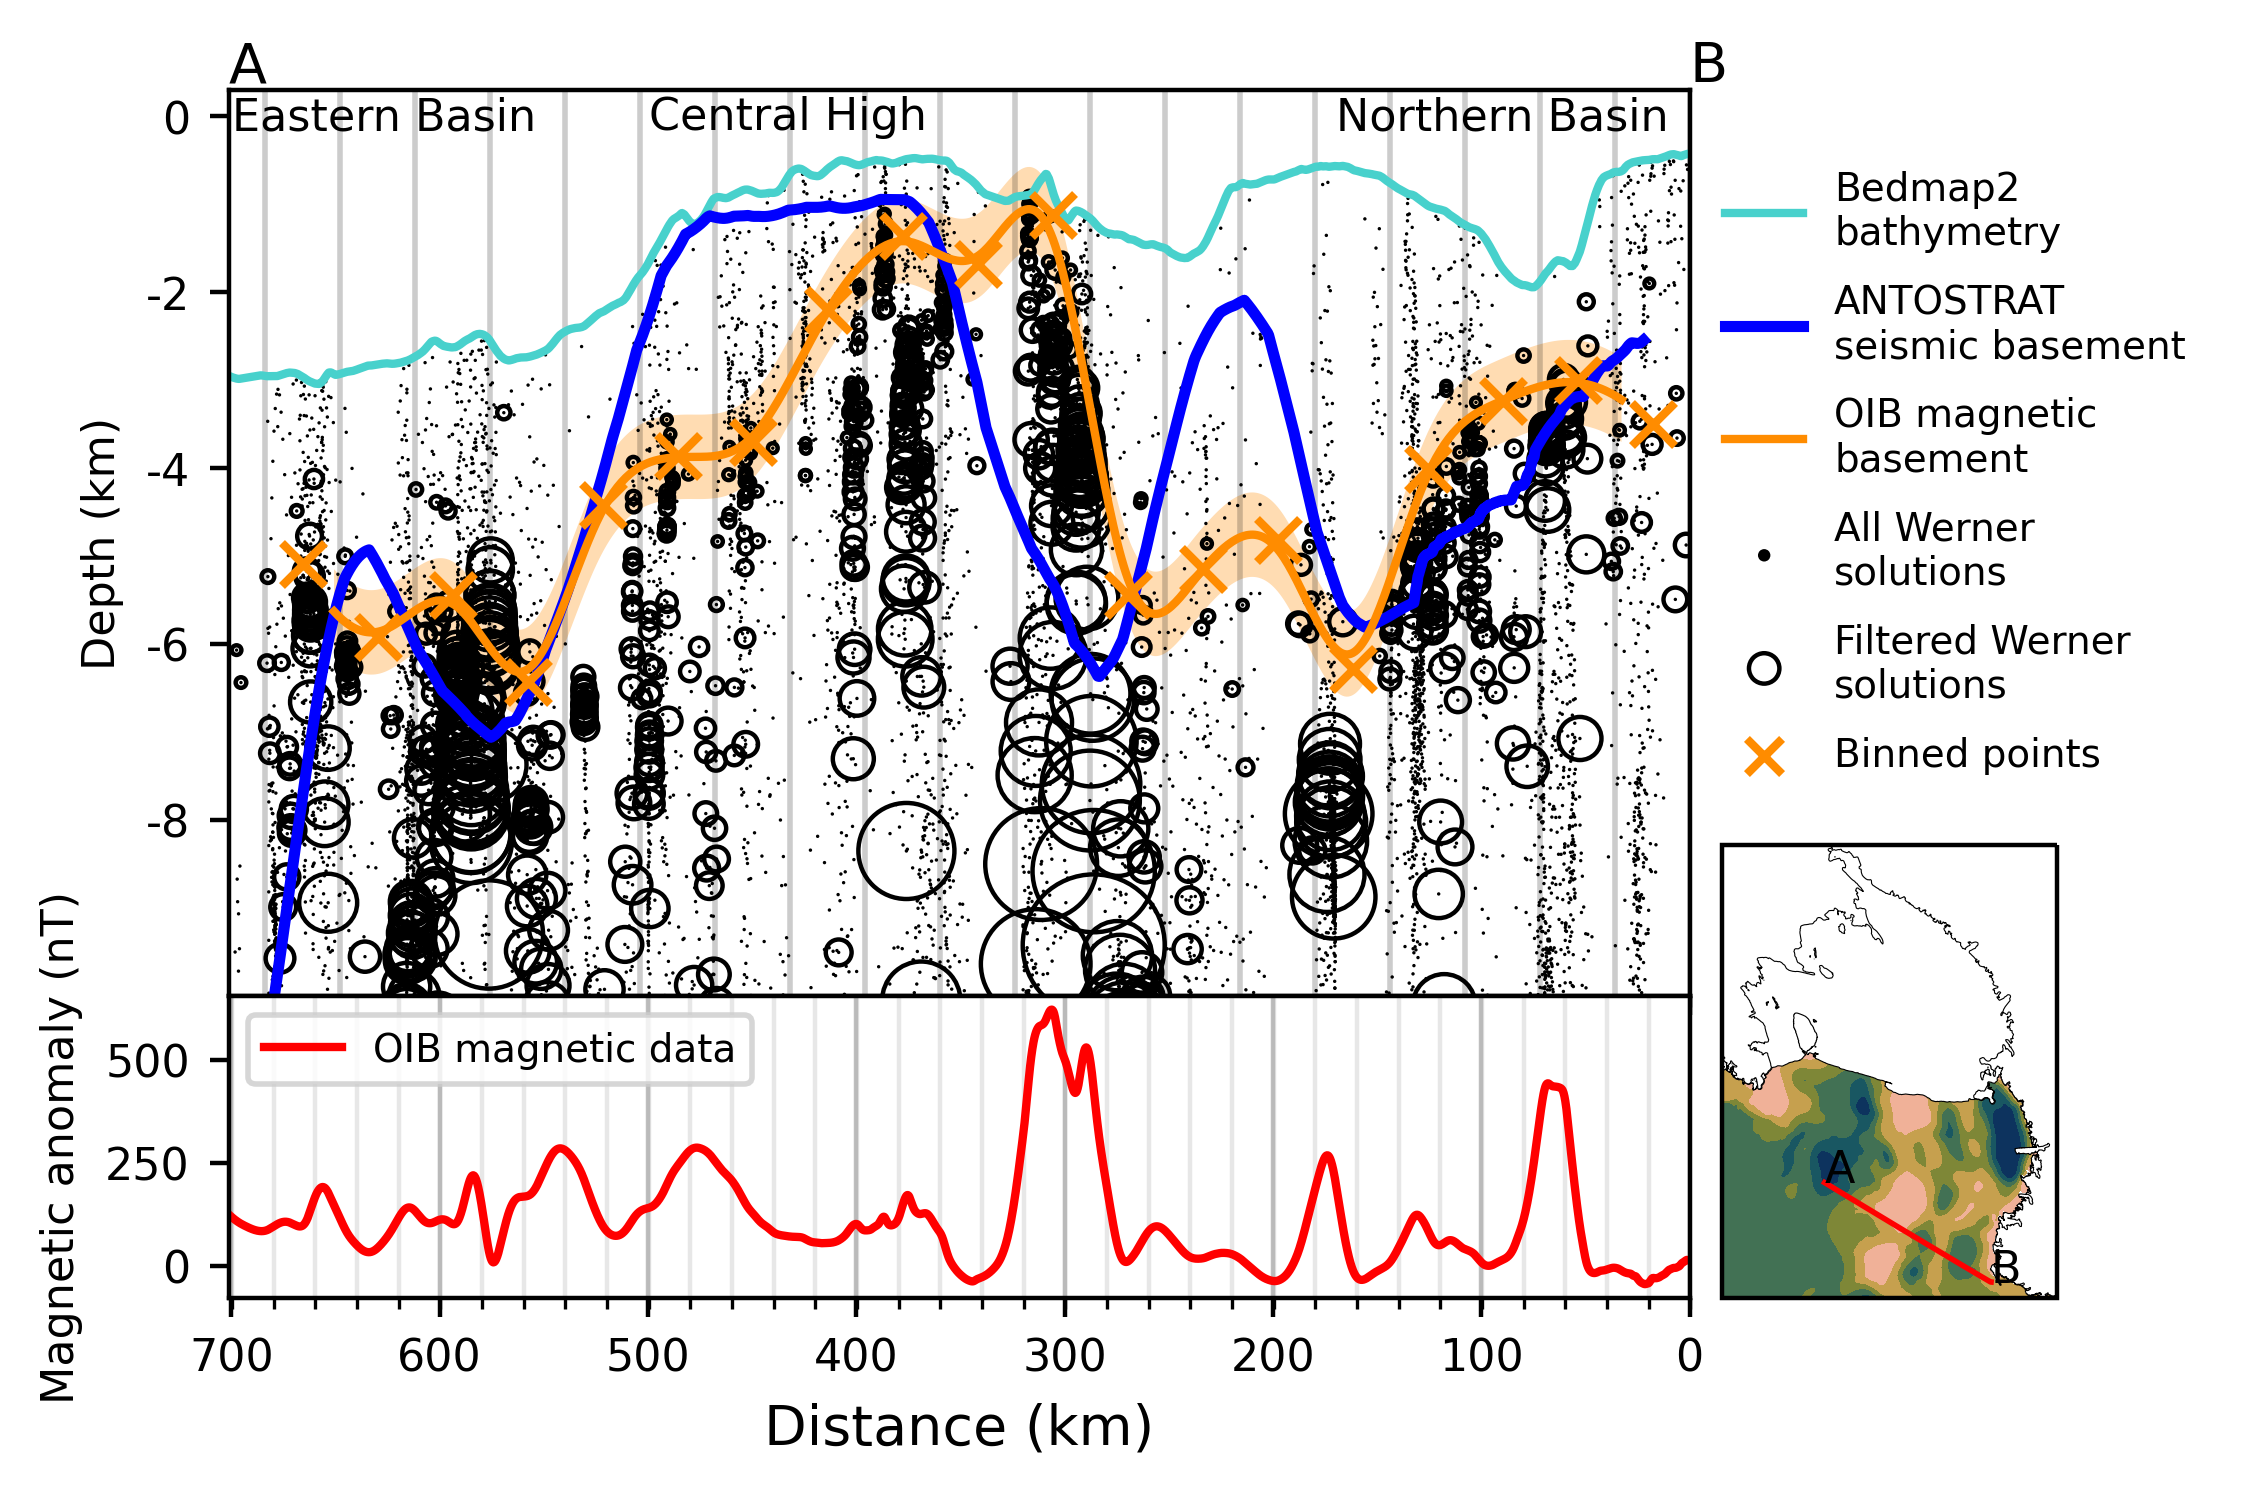
\includegraphics[width=.95\textwidth]{figures/chp2/figure_S2.png}
    \caption[OIB 403.3 magnetic and seismic basement comparison]{Ross Sea magnetic and seismic basement comparison. Operation IceBridge airborne magnetic data (lower panel) from segment 403.3 (Figure \ref{fig:chp2_Bathy_Mag}b). Small dots show Werner deconvolution solutions, which were filtered based on parameters S and W (Section \ref{appA:text_S2}) to produce black circles, which are scaled to parameter S. These circles were binned at a width equal to parameter B, shown by the vertical grey lines in the upper panel. Orange crosses show bin centres, which were fitted to a line to facilitate the comparison between the magnetic basement (orange line) and seismic basement (blue line). Orange band shows $\pm480$ m uncertainty for the basement model. Ross Sea basement features are labelled on top.}
    \label{fig:appA_S2}
\end{figure}

\begin{figure}[!ht]
    \centering
    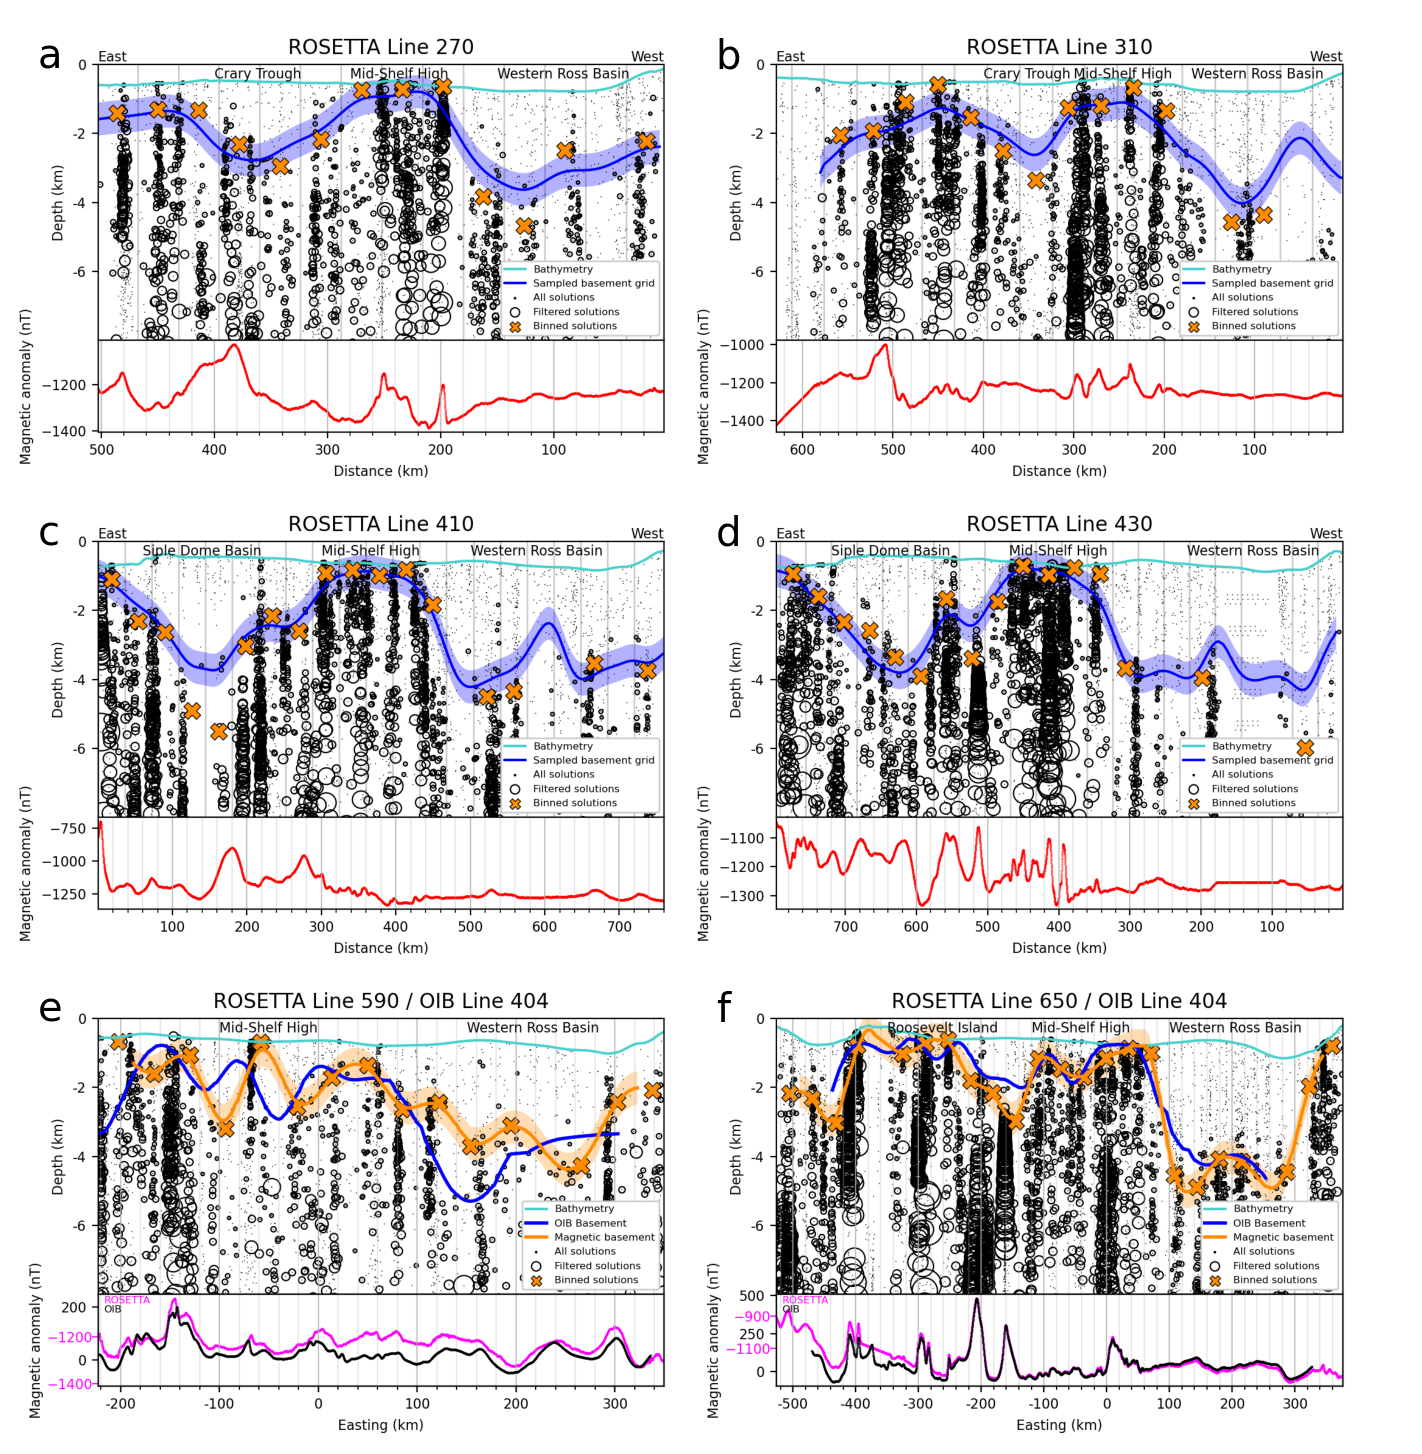
\includegraphics[width=.95\textwidth]{figures/chp2/figure_S3.png}
    \caption[Werner deconvolution solutions for ROSETTA-Ice lines]{Werner deconvolution solutions for a selection of ROSETTA-Ice lines, locations highlighted in Figure \ref{fig:appA_S4}. Bathymetry from Bedmap2 \citep{fretwellbedmap22013}. Dots, circles, and vertical grey lines same as Figure \ref{fig:appA_S2}. \textbf{a-d)} Comparison between magnetic basement before and after filtering and gridding. Orange crosses are magnetic basement solutions, shown as black dots in Figure \ref{fig:appA_S4}, and highlighted for these lines. Blue lines are magnetic basement sampled from the grid of Figure 1a, after gridding and filtering. Red lines show 258 ROSETTA-Ice magnetics data. \textbf{e-f)} Comparison between magnetic basement resulting from Werner deconvolution of coincident OIB and ROSETTA-Ice flight lines. Location is shown in Figures \ref{fig:chp2_Bathy_Mag}b and \ref{fig:appA_S4}. These two lines were used to tie the ROSETTA-Ice survey to the OIB survey (Section \ref{appA:text_S4}). Blue lines are OIB magnetic basement results, orange crosses and fitted orange lines with uncertainty bands are ROSETTA-Ice magnetic basement. ROSETTA-Ice (pink) and OIB (black) magnetics data are shown in lower panels.}
    \label{fig:appA_S3} 
\end{figure}

\begin{figure}[!ht]
    \centering
    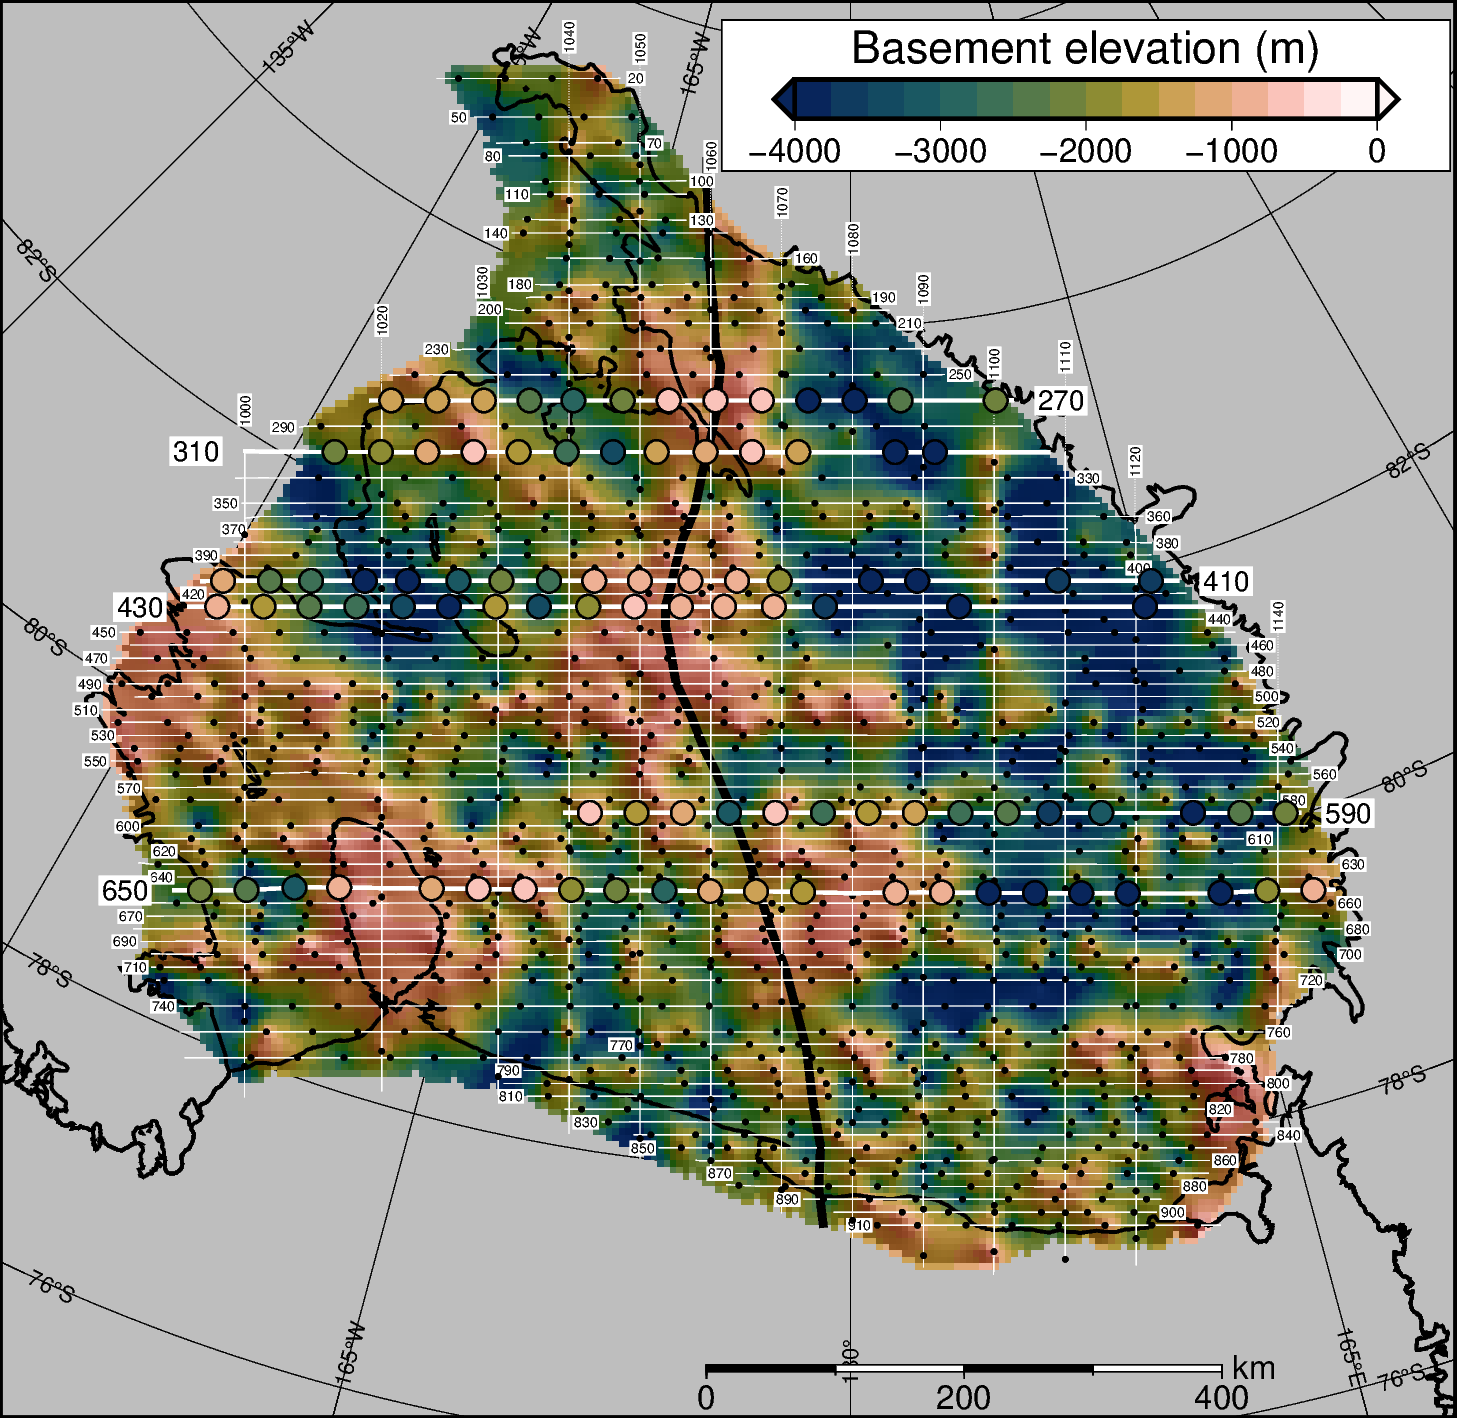
\includegraphics[width=.95\textwidth]{figures/chp2/figure_S4.png}
    \caption[Unfiltered magnetic basement and point solutions]{Unfiltered magnetic basement. Point solutions (black dots here, orange crosses in Figure \ref{fig:appA_S3}) along ROSETTA-Ice flight lines (labelled) were gridded with a 5 km cell size and a minimum curvature spline with a tension factor of 0.35. Figure \ref{fig:appA_S3} flight lines (bold white) and point solutions (coloured circles) are shown. Black line through the Mid-Shelf High shows the East-West Antarctic divide used in colorbar histograms of Figures \ref{fig:chp2_Basement_sediment} and \ref{fig:chp2_Tectonic_interpretation}a. Grounding line and coastlines in black \citep{rignoticeshelf2013}.}
    \label{fig:appA_S4}
\end{figure}

\begin{figure}[!ht]
    \centering
    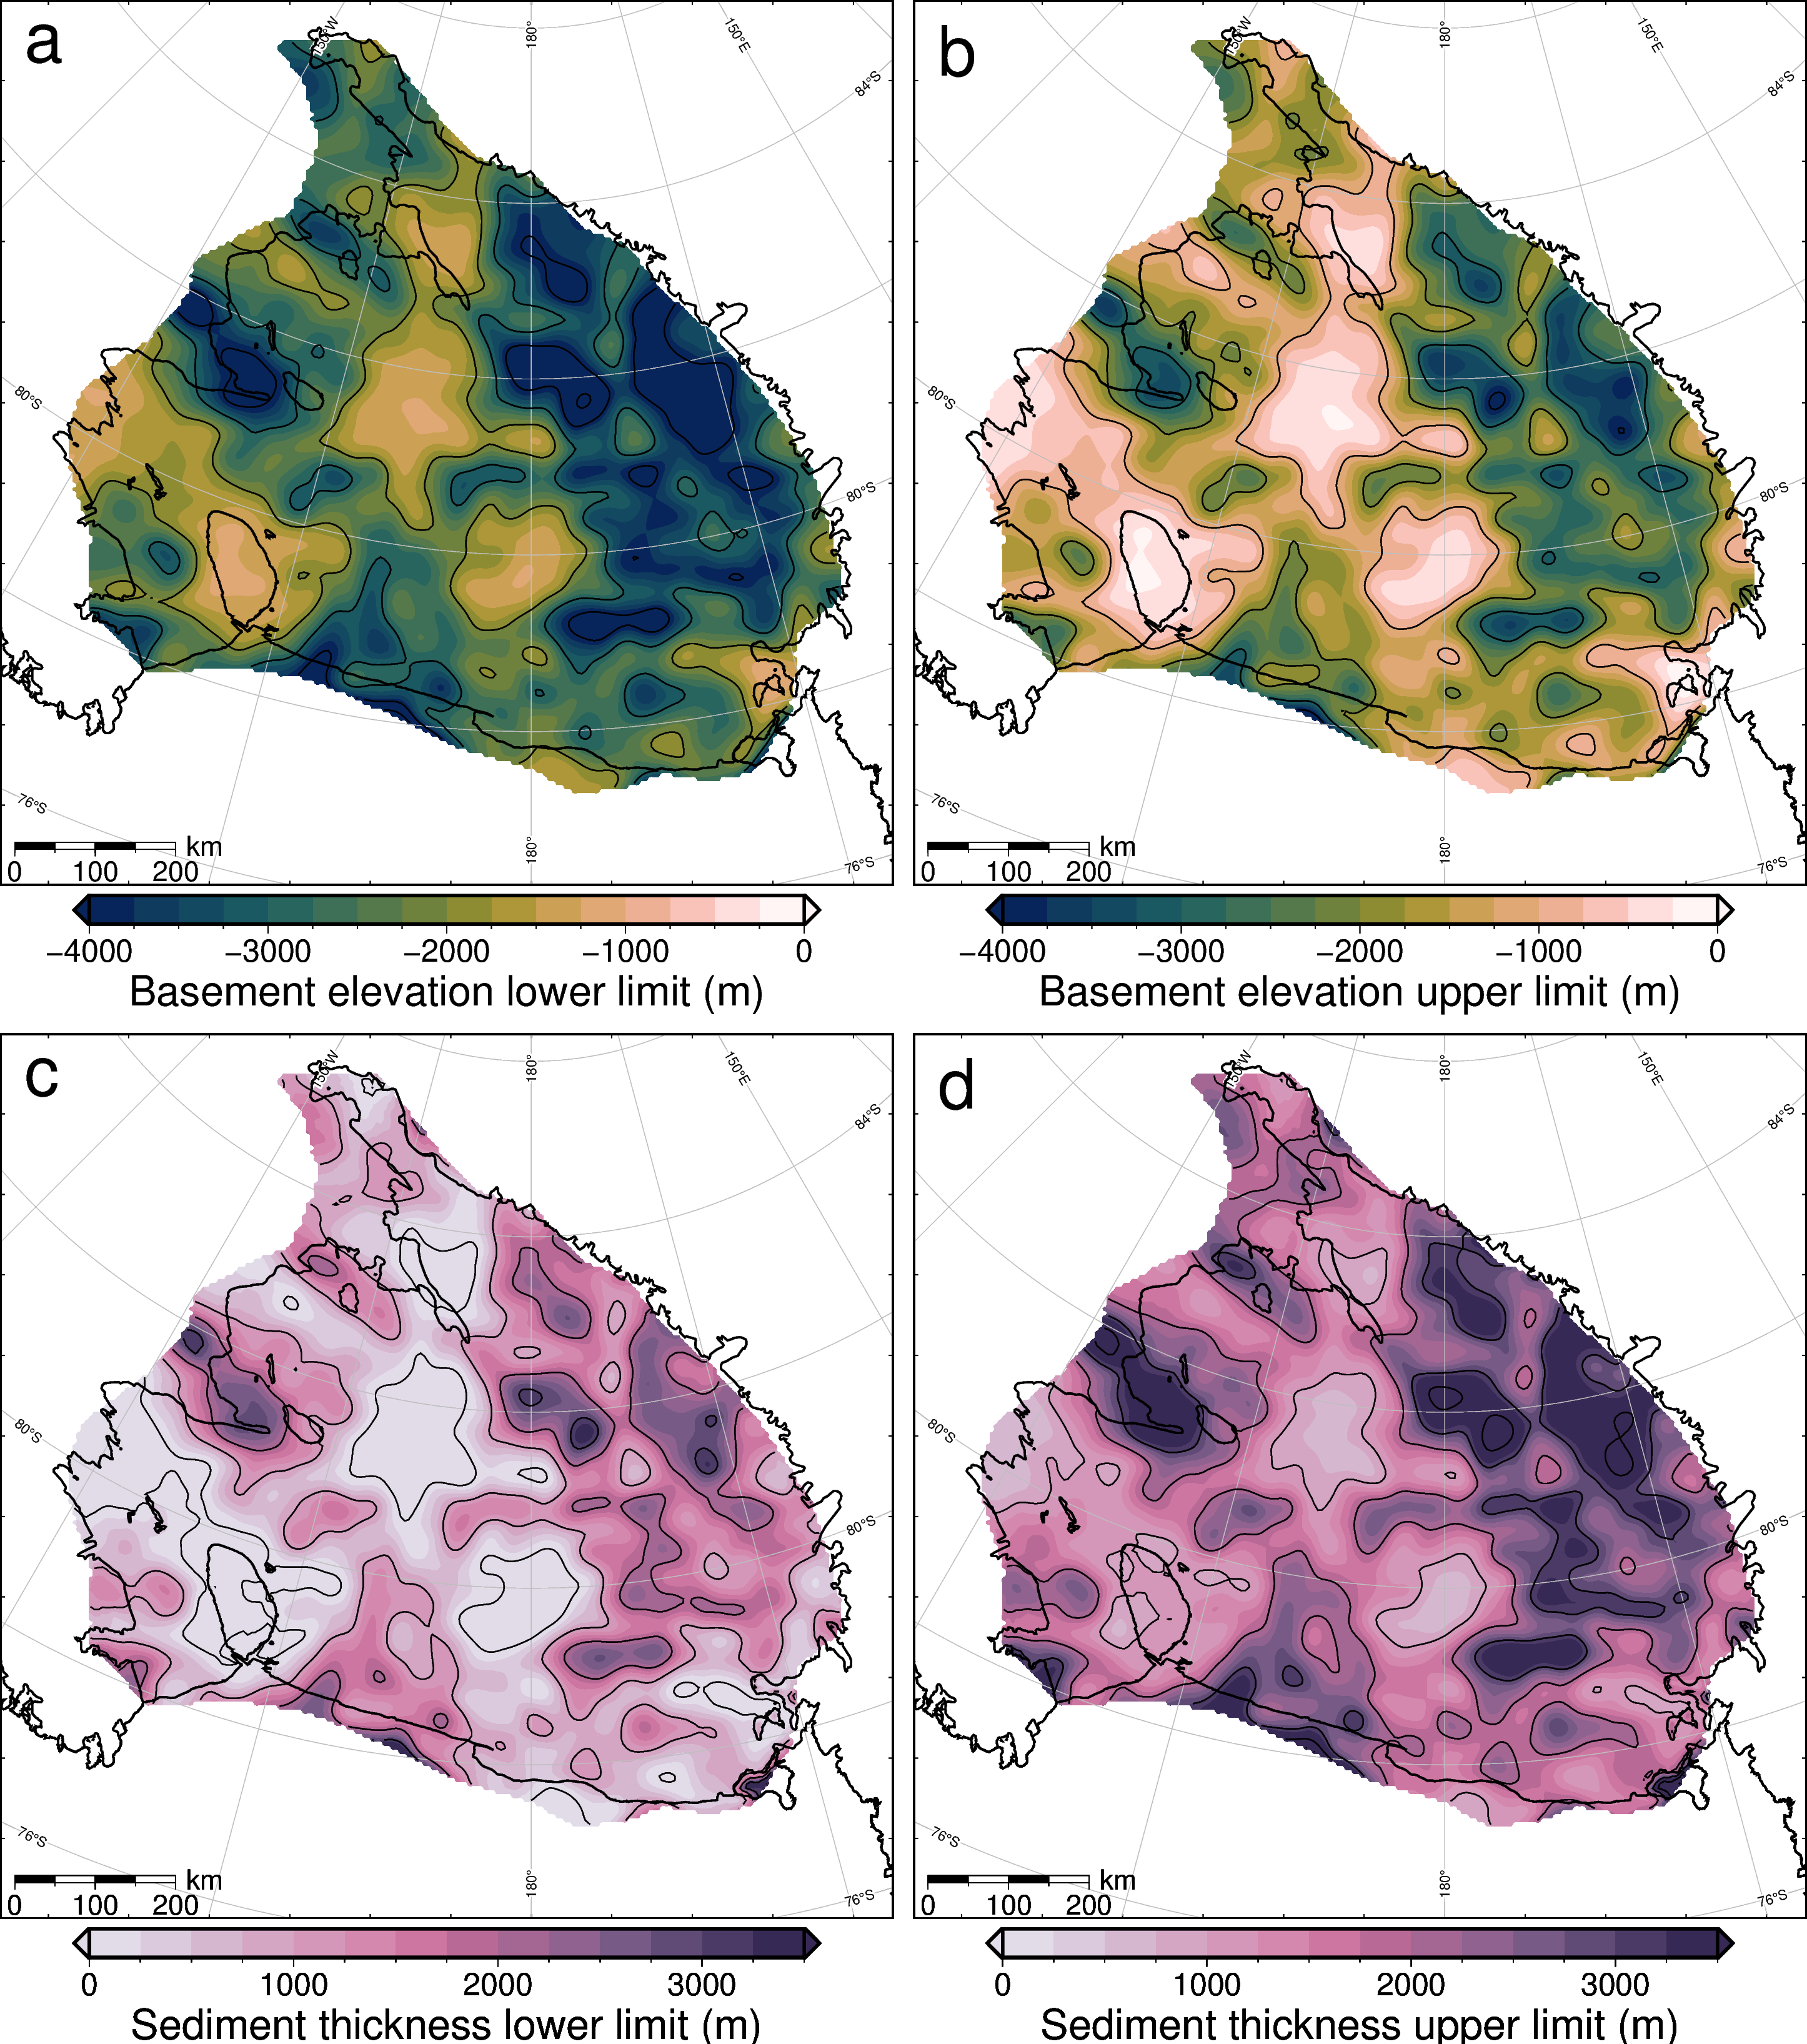
\includegraphics[width=.95\textwidth]{figures/chp2/figure_S5.png}
    \caption[Uncertainty limits of basement and sediment thickness]{Upper and lower limits of uncertainty applied to \textbf{a-b)} magnetic basement and \textbf{c-d)} sediment thickness. See Section \ref{appA:text_S7} for how these uncertainties were determined.}
    \label{fig:appA_S5}
\end{figure}

\begin{figure}[!ht]
    \centering
    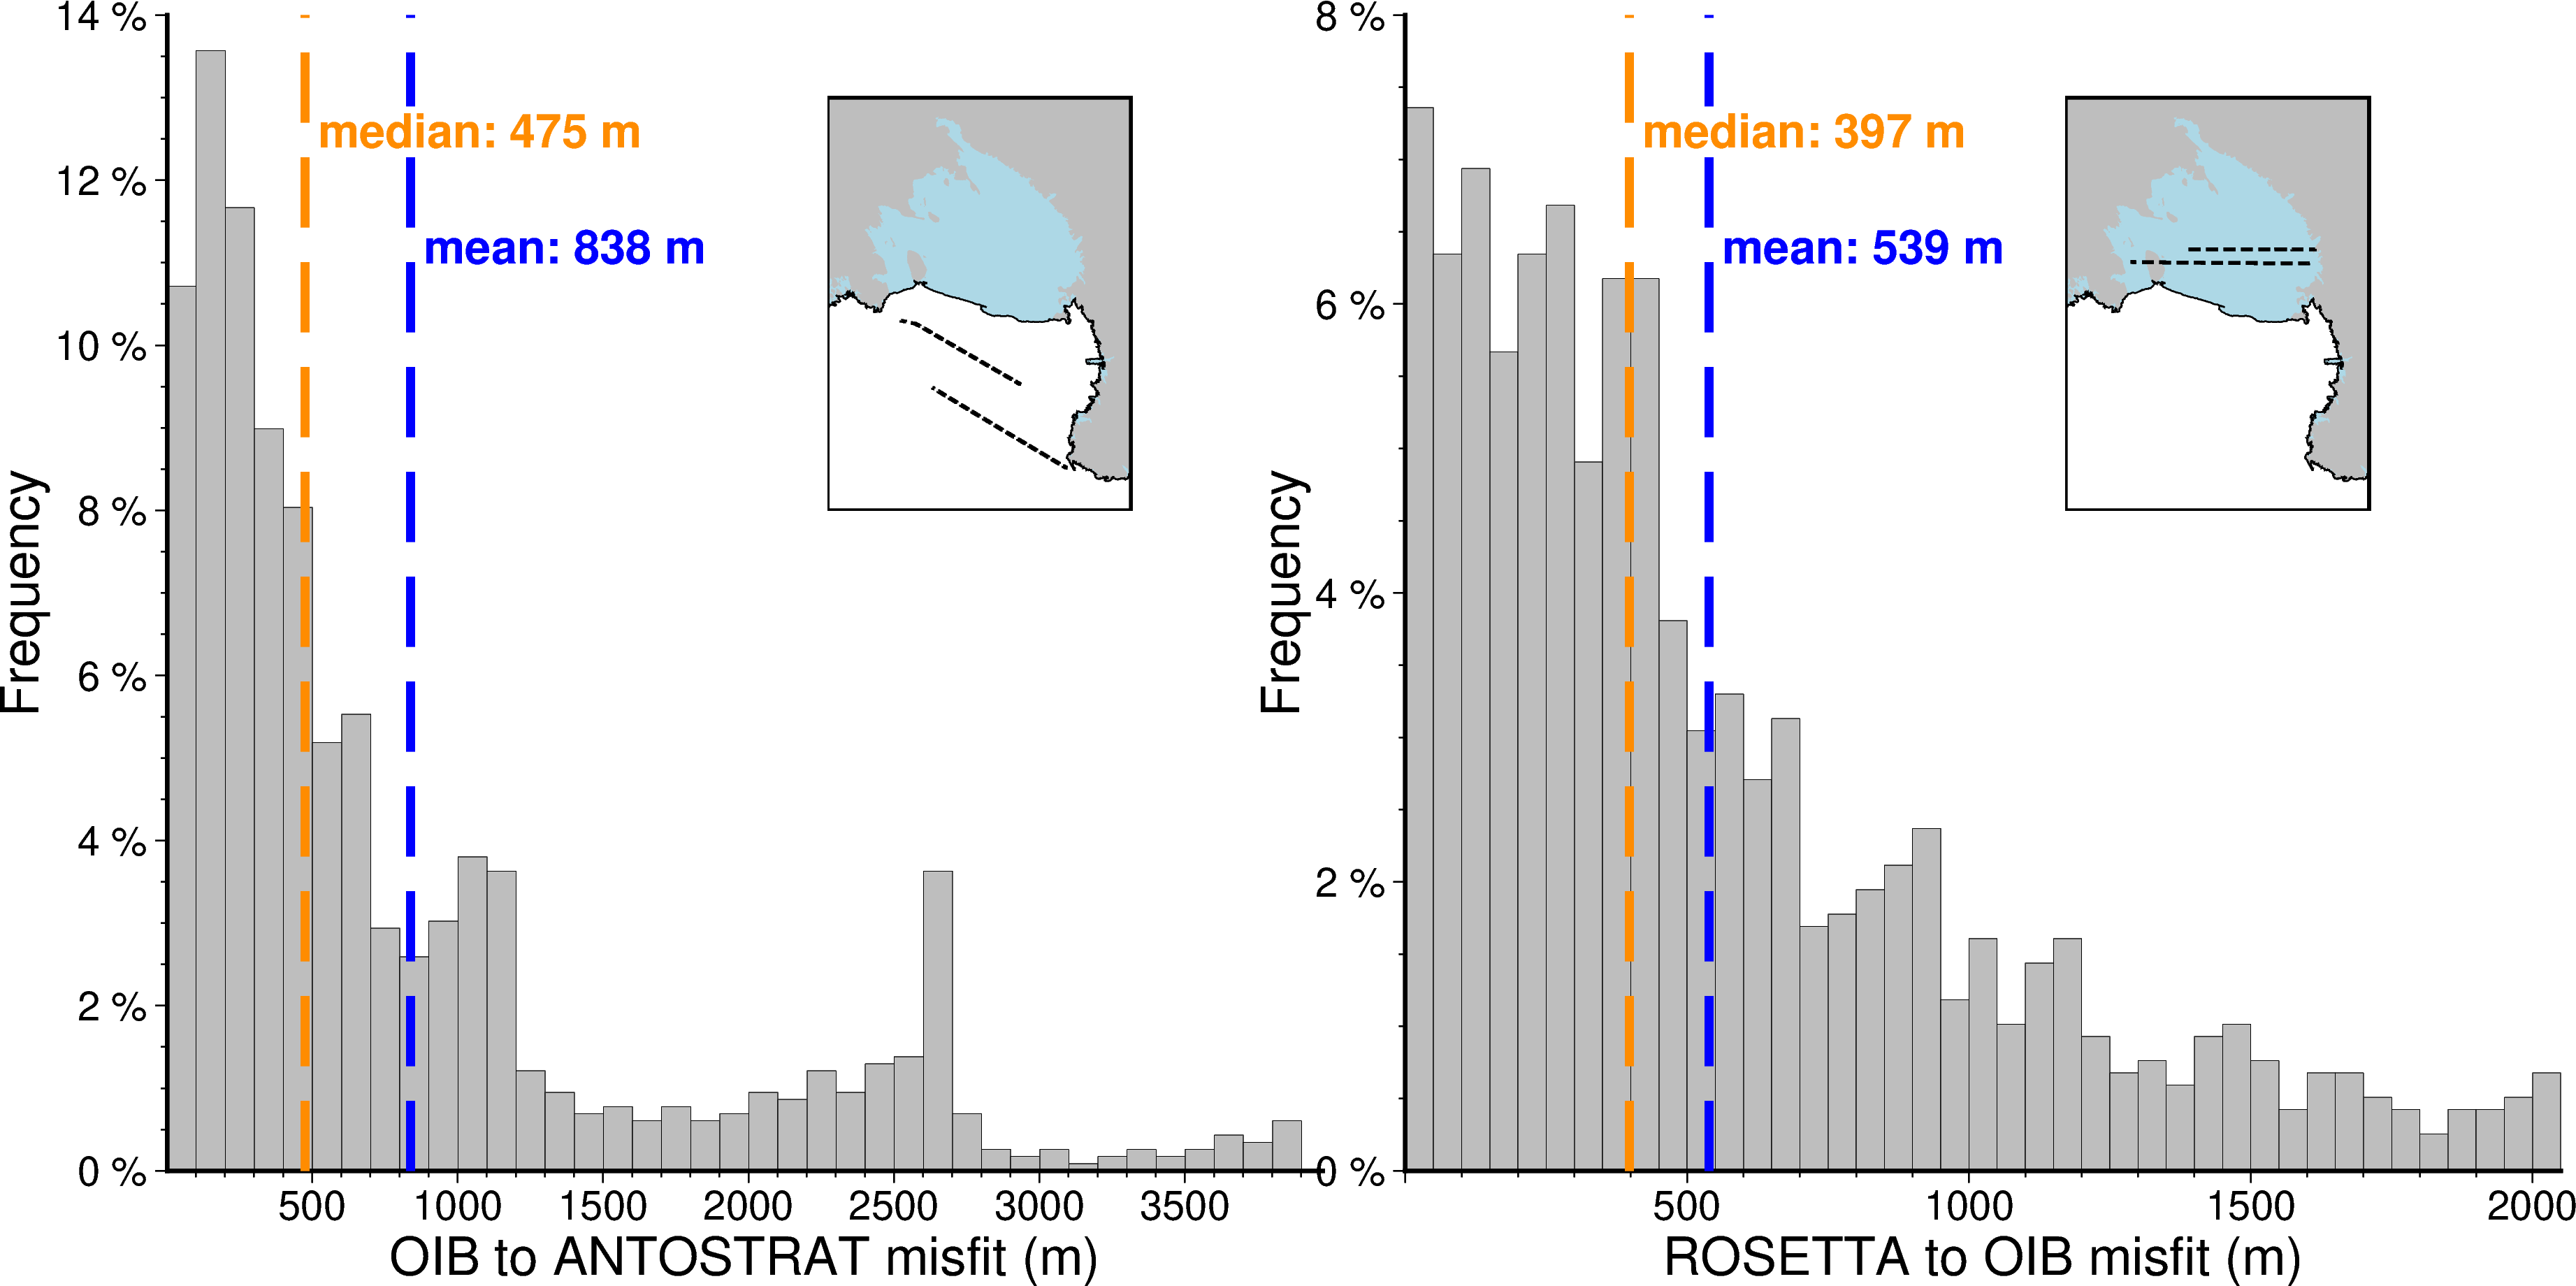
\includegraphics[width=.95\textwidth]{figures/chp2/figure_S6.png}
    \caption[Misfit distributions between magnetic and seismic basement]{Misfit distributions for comparisons between \textbf{a)} OIB magnetic basement and ANTOSTRAT seismic basement and between \textbf{b)} ROSETTA magnetic basement and OIB magnetic basement. Inset maps show the locations of flight lines. Basement models were sampled at 1 km intervals for the comparison.}
    \label{fig:appA_S6} 
\end{figure}

\clearpage

 
 




\chapter{} \label{appendix:B}
This appendix section provides supplementary information to Chapter \ref{ch:3}. 

\section{Synthetic inversion with a regional field} \label{appendix:B:simple_regional_inversion}

\paragraph*{Regional separation techniques}

Figure \ref{fig:appB_simple_regional_comparison_profile} shows profiles comparing the various regional separation techniques shown in Figure \ref{fig:chp3_simple_regional_comparison} of Chapter \ref{ch:3}.

\begin{figure}[!ht]
    \centering
    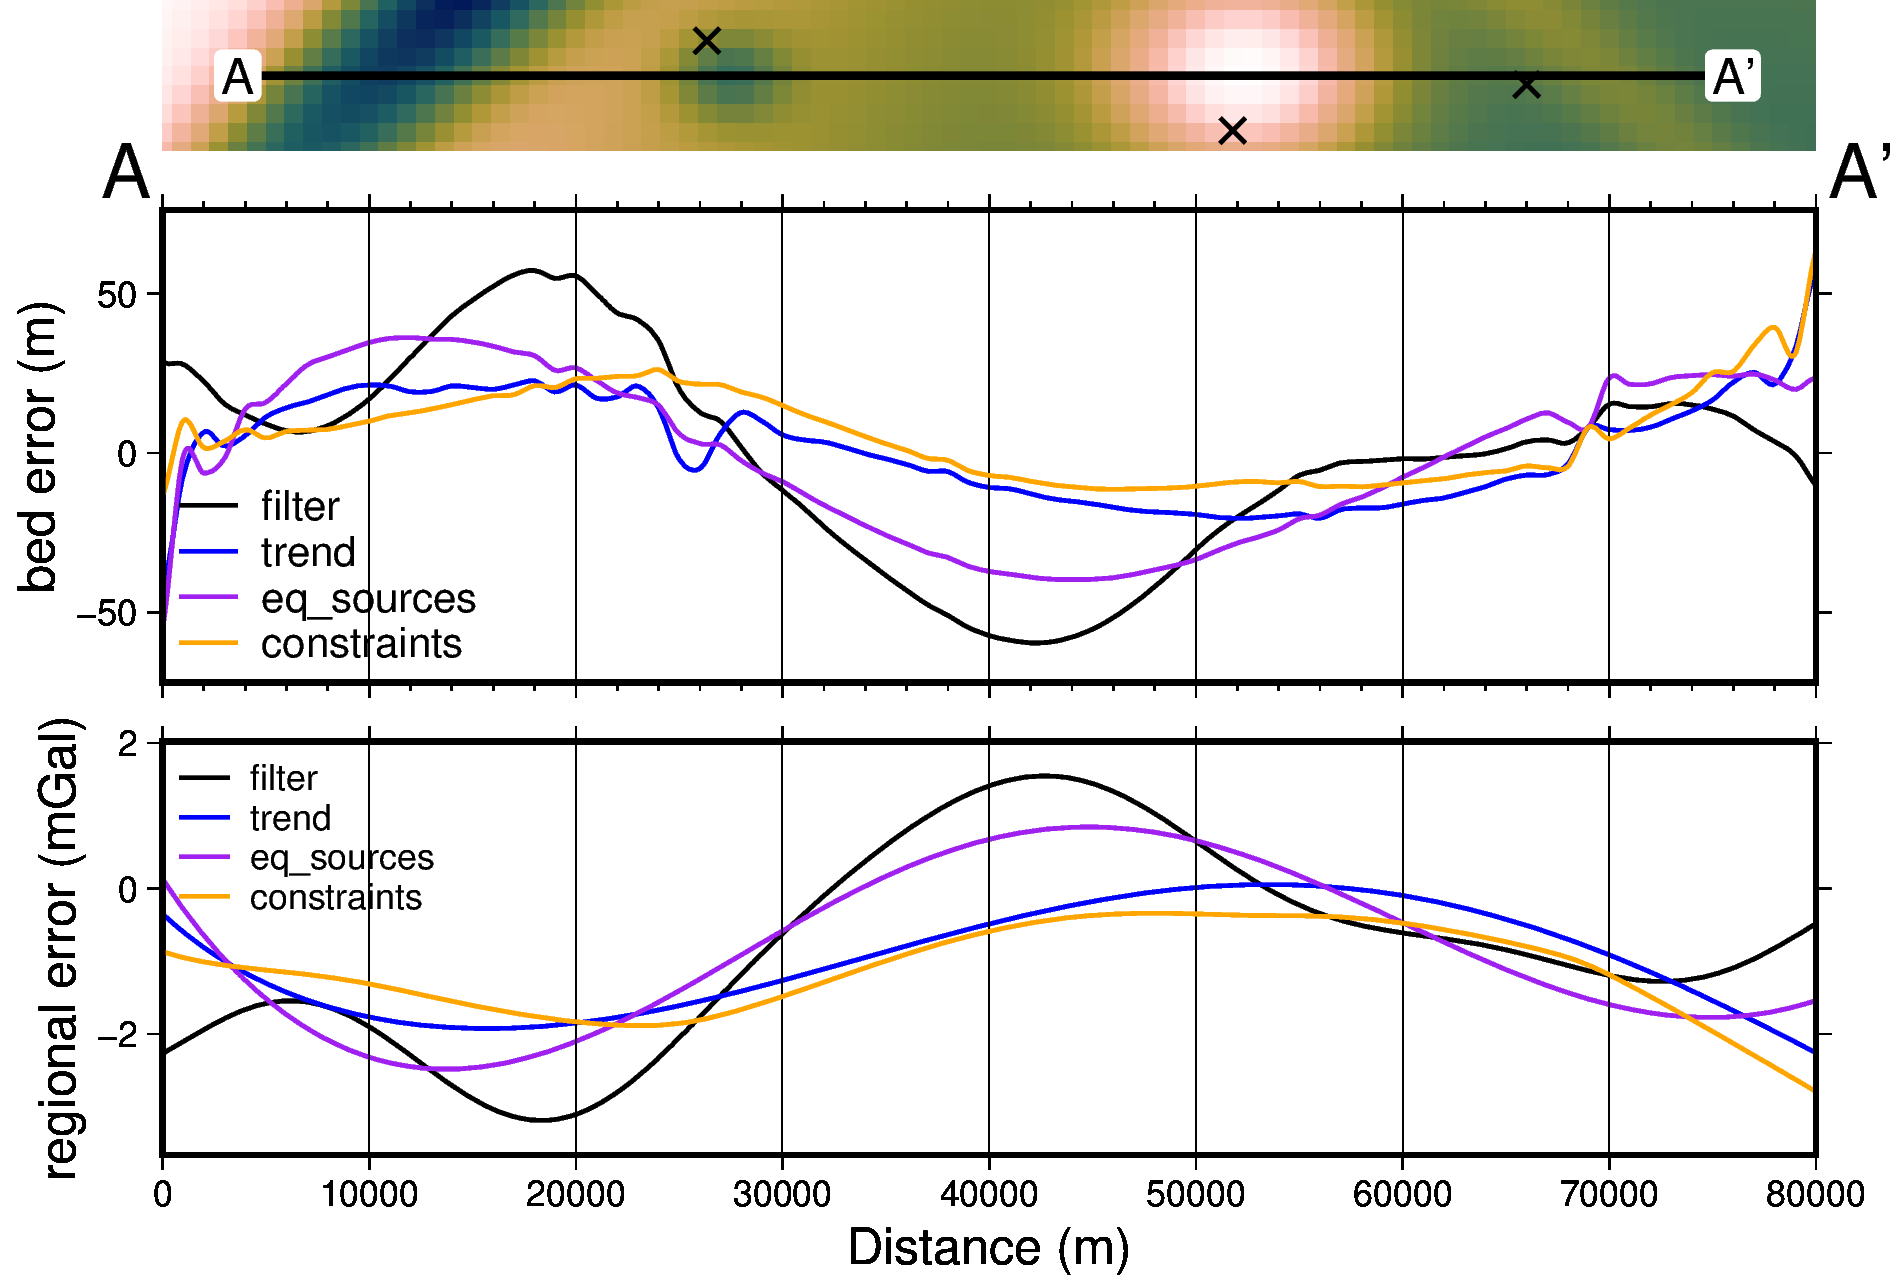
\includegraphics[width=.95\textwidth]{figures/chp3/chp3_simple_regional_comparison_profiles.png}
    \caption[Comparison of four methods of regional separation]{Comparison of four methods of regional separation. \textbf{Upper panel} shows the error in the inverted bathymetry models for each method. \textbf{Lower panel} shows the errors in the regional field estimation of each method. Profile location shown at the top.}
    \label{fig:appB_simple_regional_comparison_profile}
\end{figure}

\paragraph*{Constraint point minimization gridding techniques}

Figure \ref{fig:appB_simple_regional_comparison_profile} shows profiles comparing the various gridding techniques for the constraint point minimization regional separation method. These various gridding techniques are shown in map view in Figure \ref{fig:chp3_simple_regional_gridding_comparison} of Chapter \ref{ch:3}.

\begin{figure}[!ht]
    \centering
    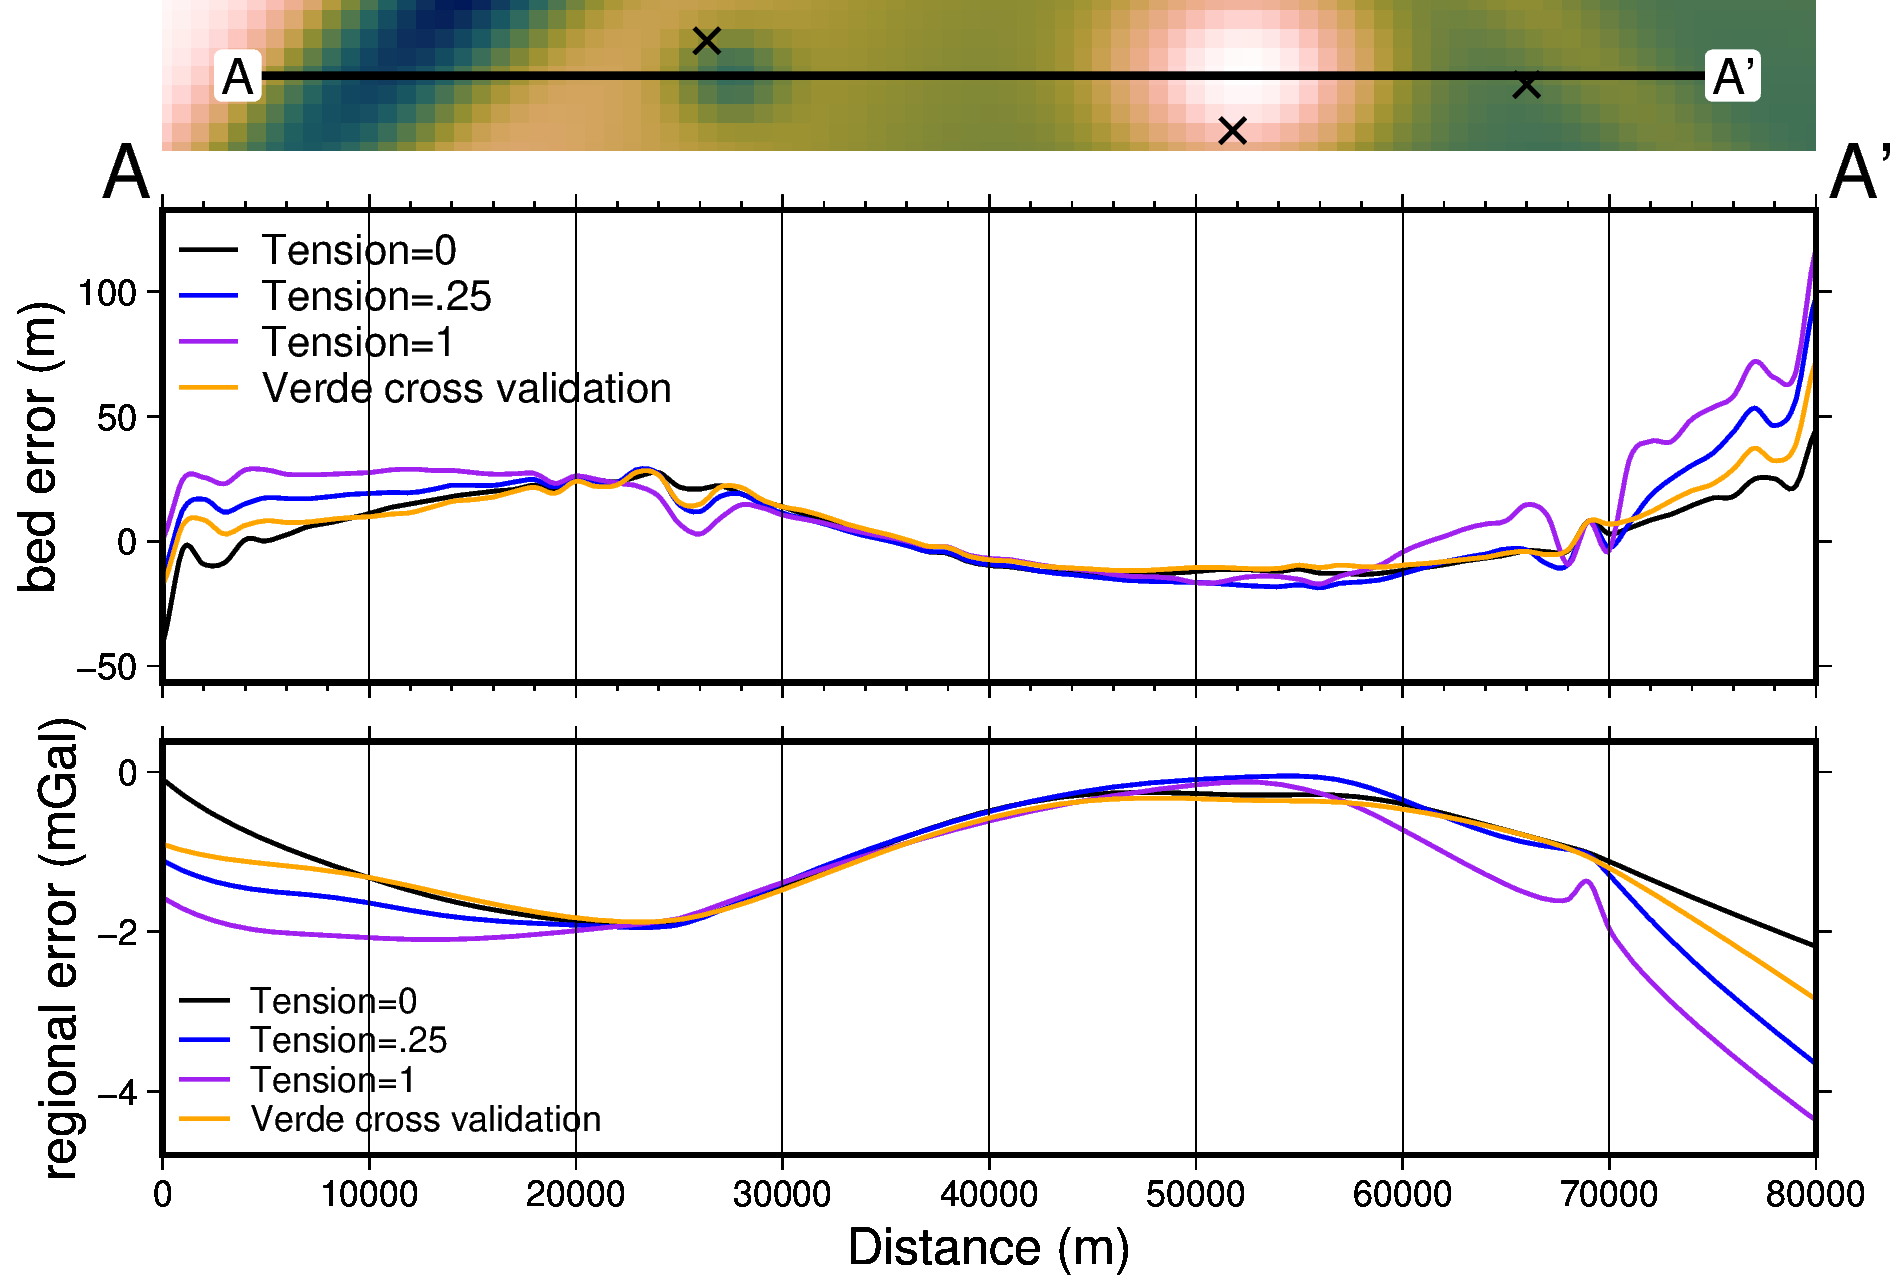
\includegraphics[width=.95\textwidth]{figures/chp3/chp3_simple_regional_gridding_comparison_profiles.png}
    \caption[Constraint point minimization gridding comparison profiles]{Comparison of gridding techniques for the constraint point minimization method of regional separation. \textbf{Upper panel} shows the error in the inverted bathymetry models for each method. \textbf{Lower panel} shows the errors in the regional field estimation of each method. Profile location shown at the top.}
    \label{fig:appB_simple_regional_gridding_comparison_profile}
\end{figure}

\paragraph*{Added noise}

Here, we repeat the inversion from Section \ref{chp3:simple_regional_model} with noise added to the observed gravity data. Noise was from a Gaussian distribution with a mean of 0 and a standard deviation of 2\% of the max absolute values of the data, equating to 0.24 mGal. The cross-validation curve and a profile across the inverted bathymetry as shown in Figure \ref{fig:appB_simple_regional_noise_CV_and_profile}. The inverted bathymetry and difference with the true bathymetry as shown in Figure \ref{fig:appB_simple_regional_noise_results}. The error in the inverted bathymetry is compared to the error in the regional field estimation in Figure \ref{fig:appB_simple_regional_noise_bed_error}.

\begin{figure}[!ht]
  \centering
    \begin{subfigure}[t]{.40\textwidth}
        \centering
        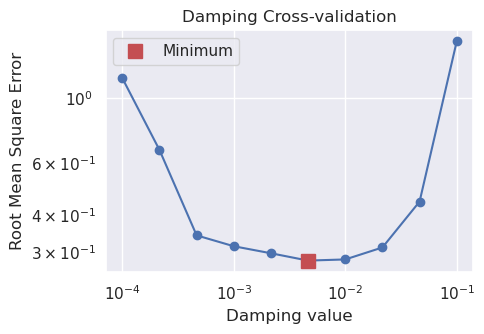
\includegraphics[width=\textwidth]{figures/chp3/chp3_simple_regional_noise_CV.png}
        \caption{}
    \end{subfigure}
    \begin{subfigure}[t]{.58\textwidth}
        \centering
        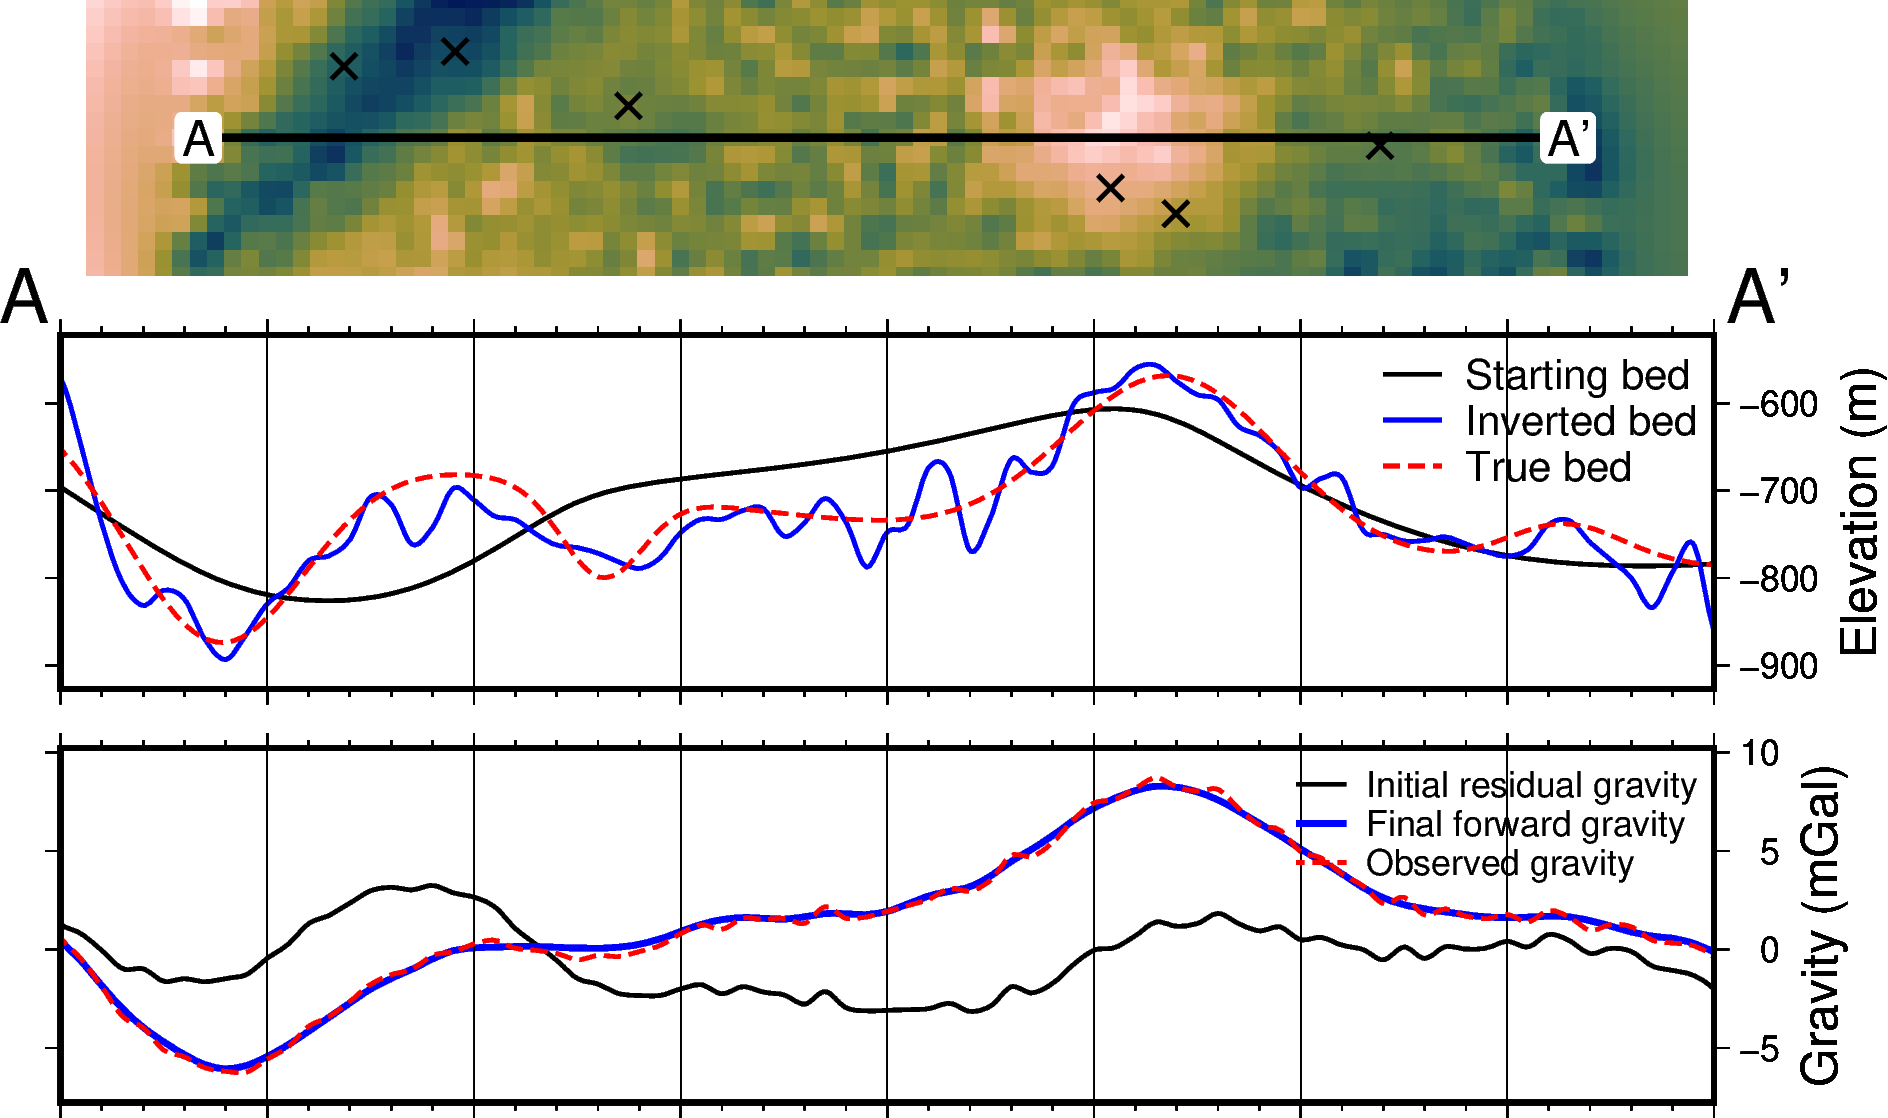
\includegraphics[width=\textwidth]{figures/chp3/chp3_simple_regional_noise_profile.png}
        \caption{}
    \end{subfigure}
  \caption[Synthetic inversion with regional and noise, CV and profile]{Cross-validation and profiles for the simple synthetic inversion with a regional component removed and 2\% noise added to the observed gravity data. a) Cross-validation curve showing the optimal damping parameter (red square). b) 2D profile of the inversion results. The top panel shows profile location and constraint points (black crosses). The middle panel contains topographic profiles of the starting, inverted, and true bathymetries. The bottom panel contains gravity anomaly profiles.}
    \label{fig:appB_simple_regional_noise_CV_and_profile}
\end{figure}

\begin{figure}[!ht]
    \centering
    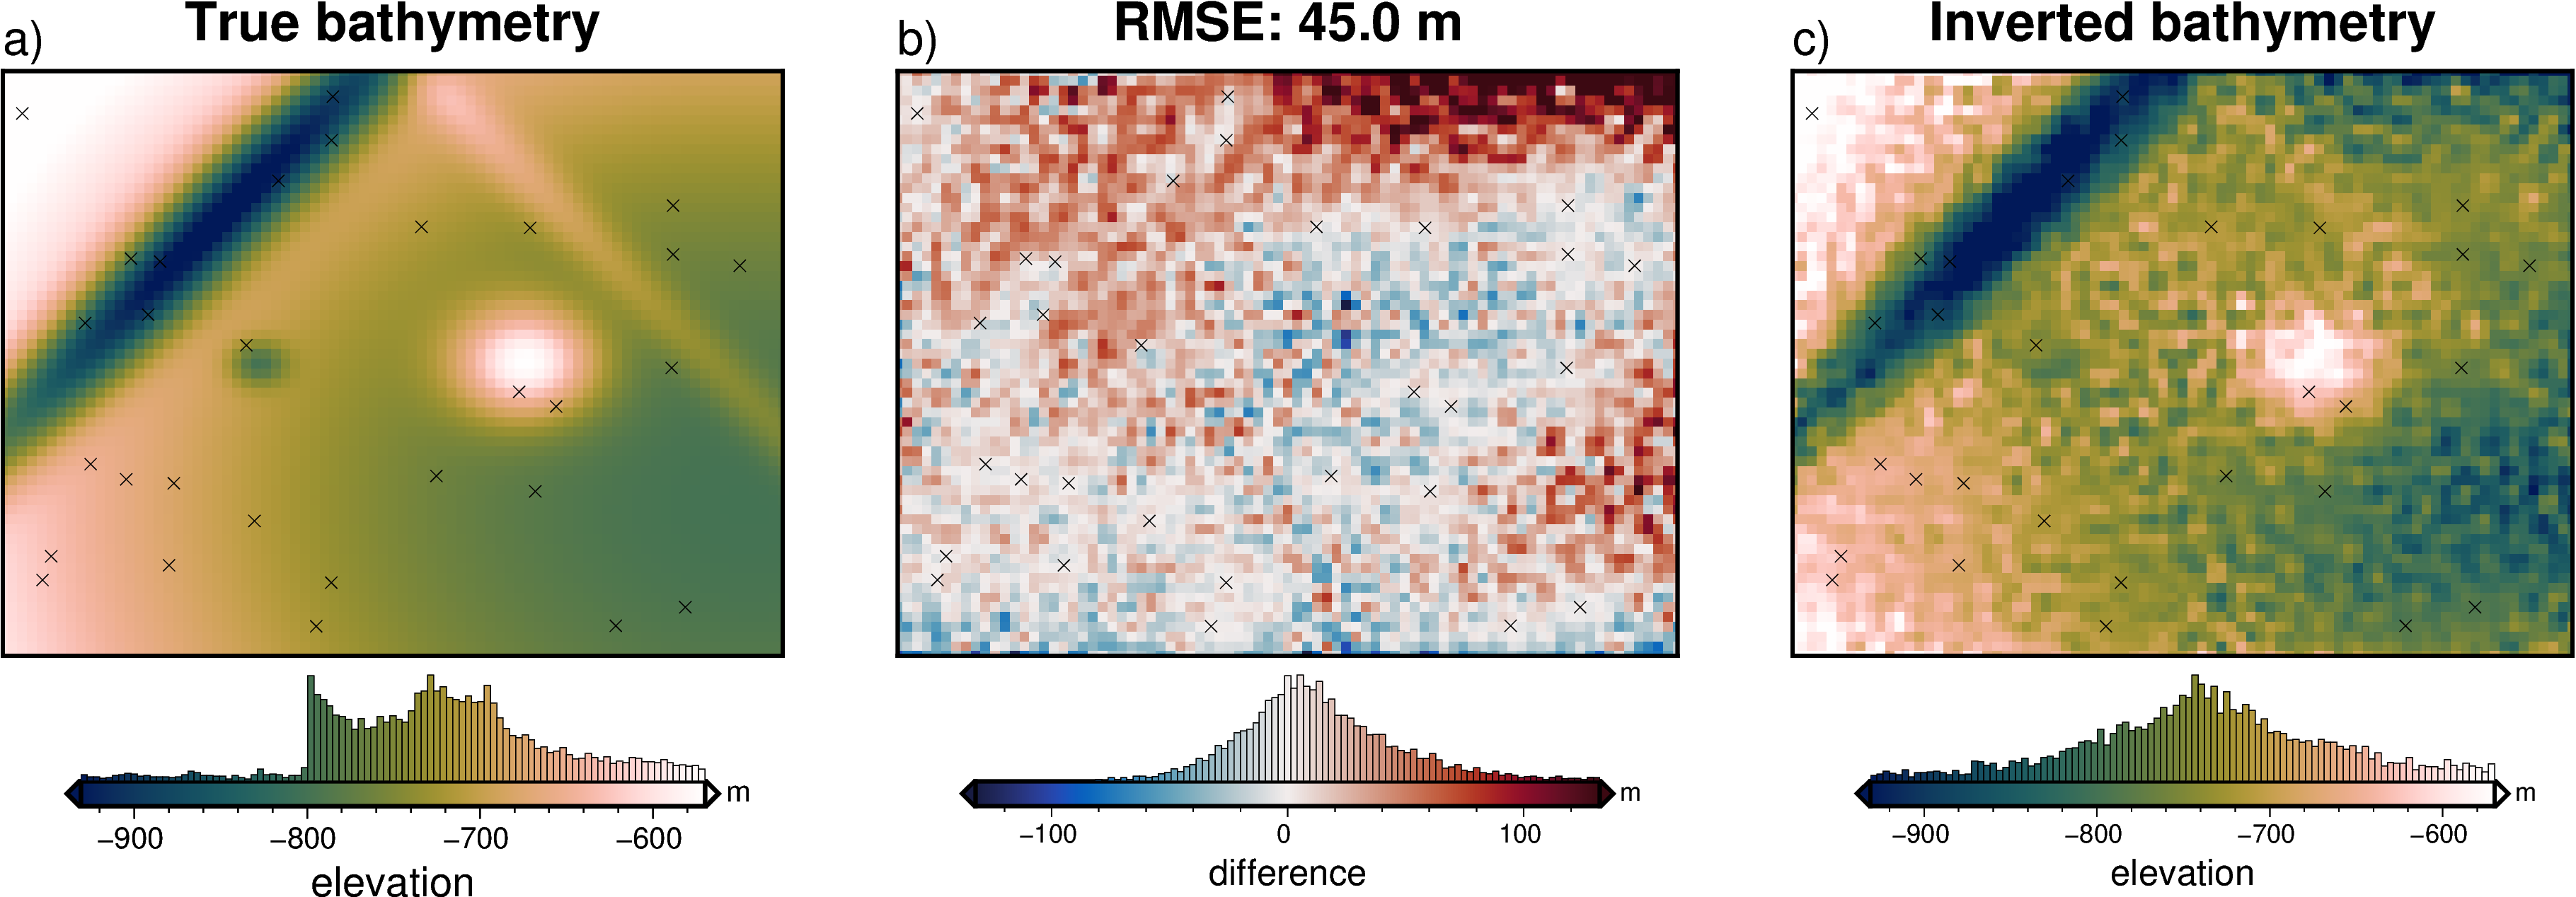
\includegraphics[width=.95\textwidth]{figures/chp3/chp3_simple_regional_noise_results.png}
    \caption[Synthetic inversion with regional and noise, results]{Simple synthetic model inversion with a removed regional component and noise contamination. a) True bathymetry, b) difference between a) and c), c) final inverted bathymetry. Black crosses are constraint points. The RMS difference with the true bathymetry at these constraints is 2 m.}
    \label{fig:appB_simple_regional_noise_results}
\end{figure}

\begin{figure}[!ht]
    \centering
    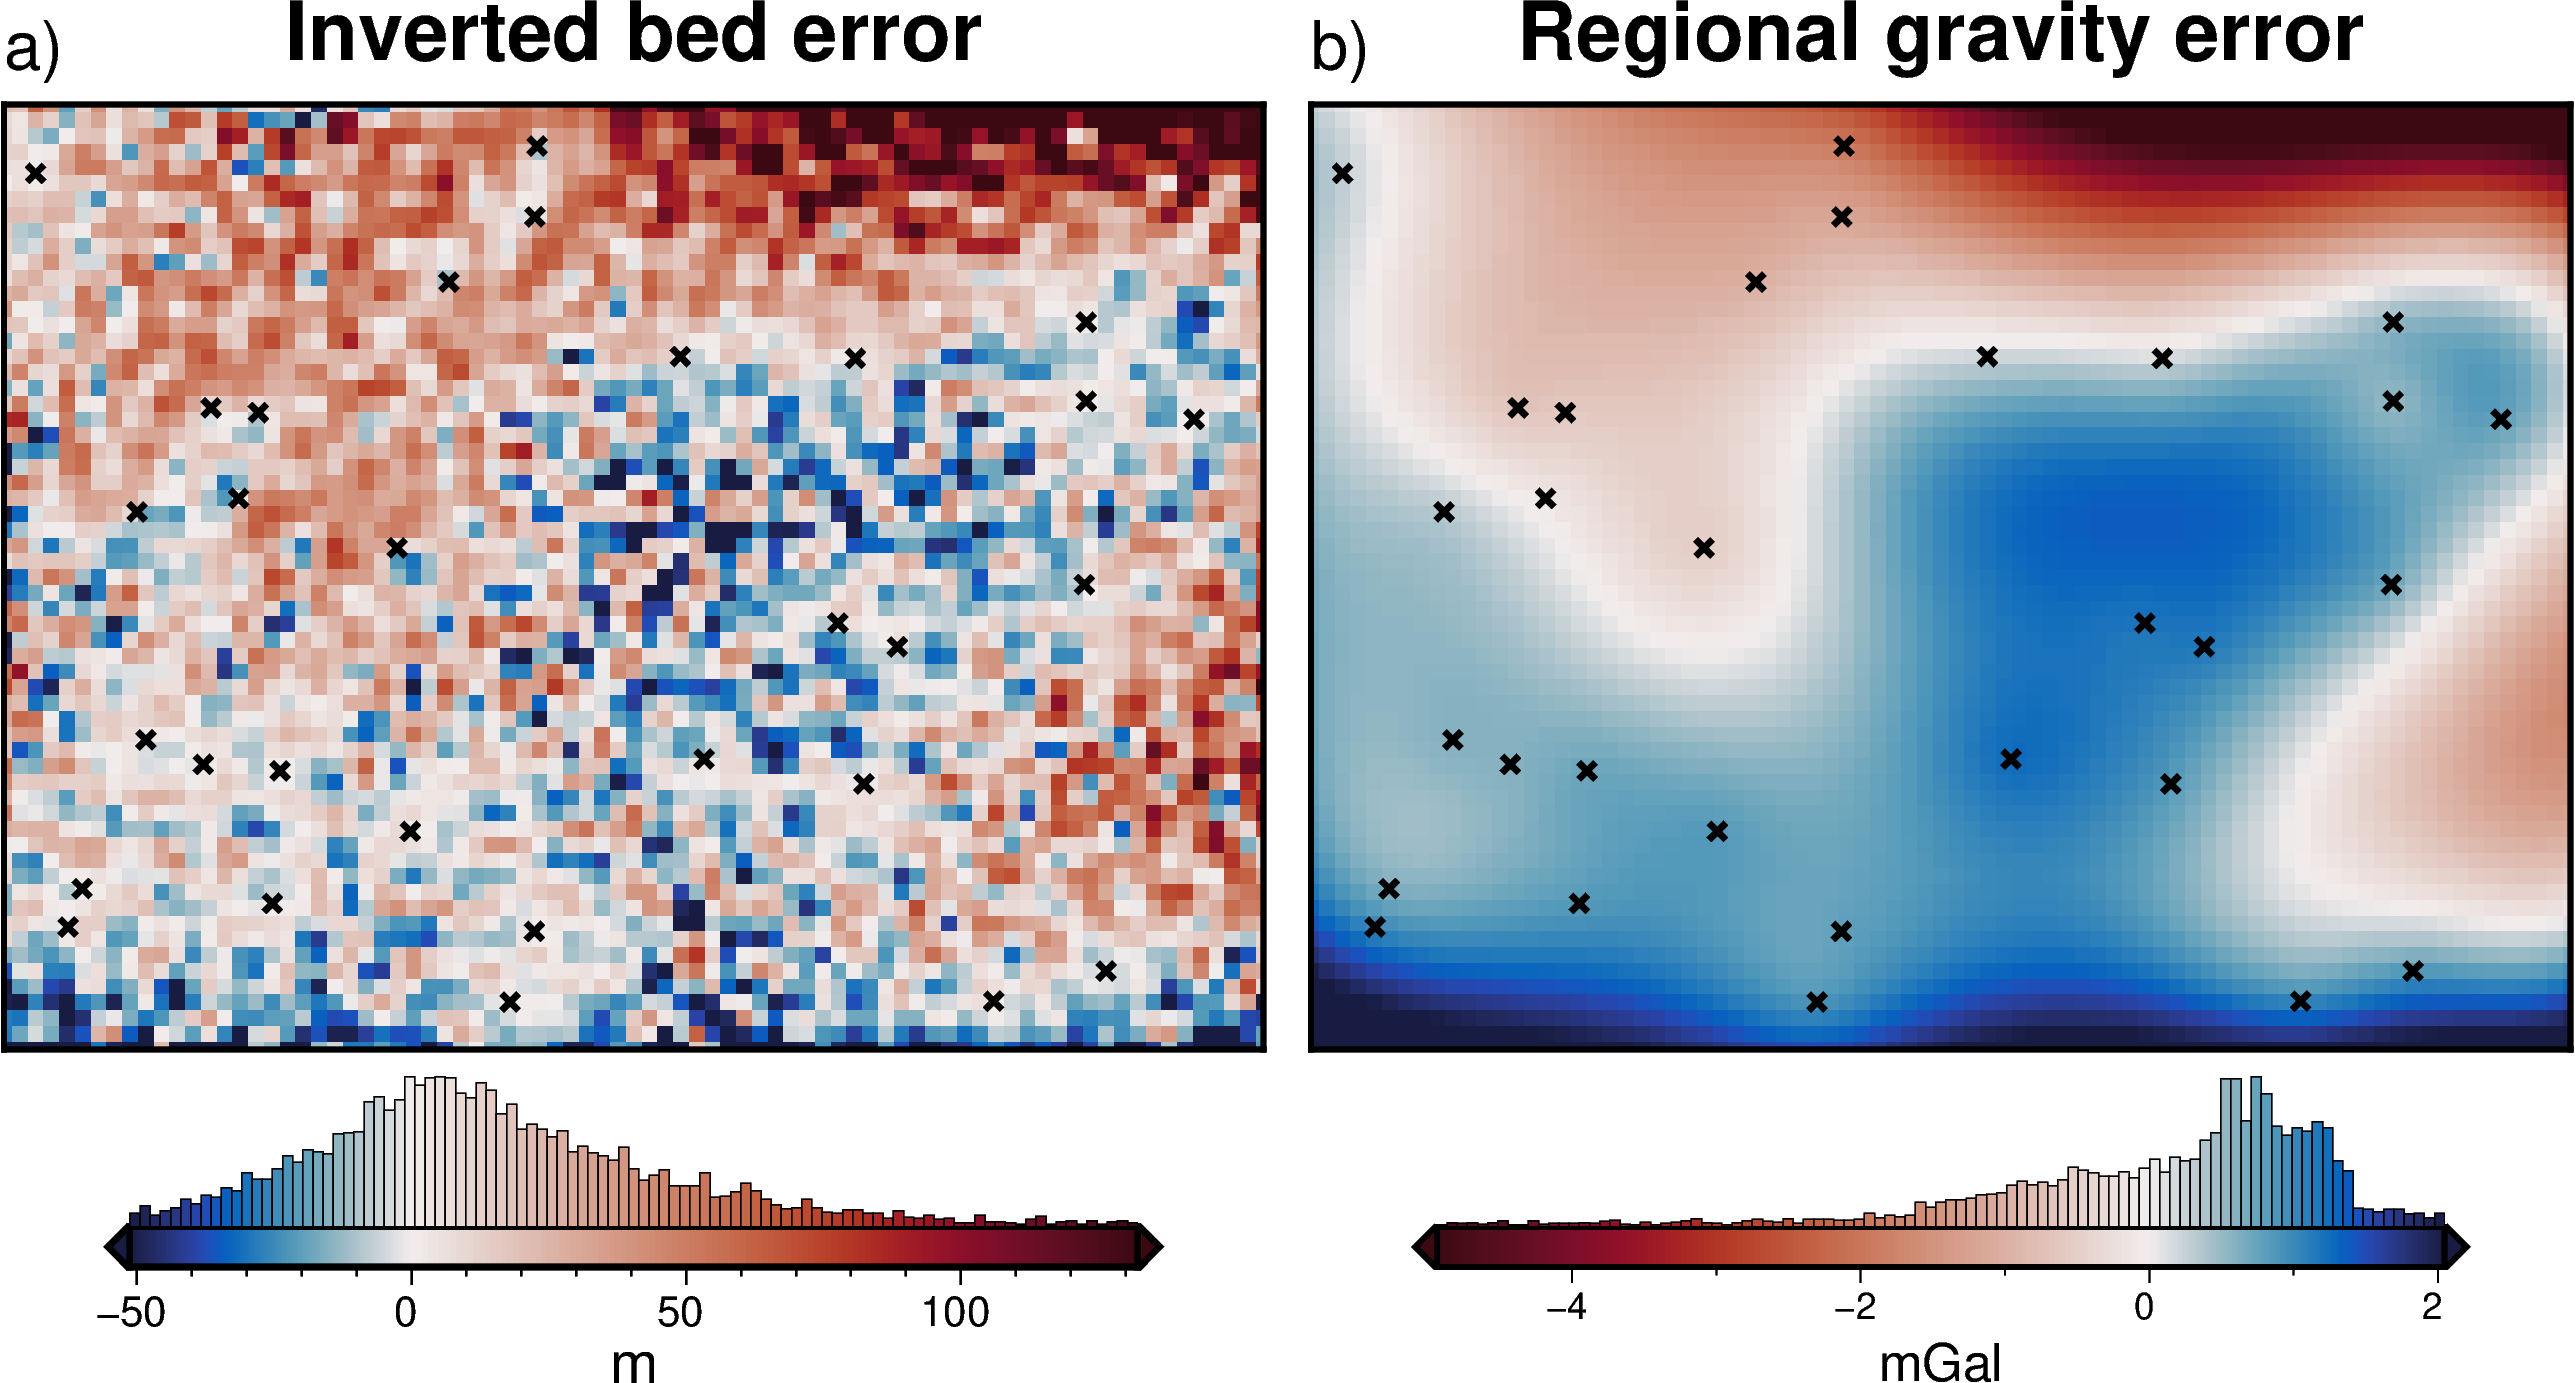
\includegraphics[width=.7\textwidth]{figures/chp3/chp3_simple_regional_noise_bed_error.png}
    \caption[Inversion and regional error for model with regional and noise]{Source of inverted bathymetry error for model with regional field and noise. a) Inverted bathymetry error from Figure \ref{fig:chp3_simple_regional_results}b. b) Error in the estimation of the regional component of gravity from comparison with the true regional component (Figure \ref{fig:chp3_simple_regional_gravity}b). Black cross show constraint points. Colourmaps are opposed to highlight the similarities and the mean has been removed from the regional error.}
    \label{fig:appB_simple_regional_noise_bed_error}
\end{figure}

\paragraph*{Lower-resolution gravity survey}

This same inversion is now repeated with a lower-resolution gravity survey. Instead of the original 1 km survey grid, a 4 km grid is used. 

\begin{figure}[!ht]
  \centering
    \begin{subfigure}[t]{.40\textwidth}
        \centering
        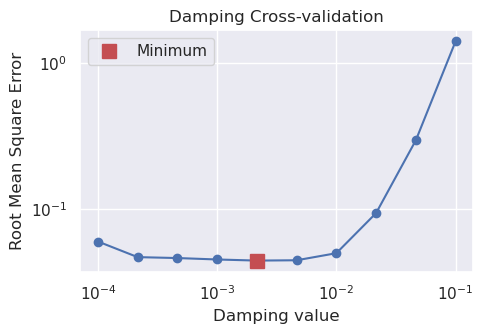
\includegraphics[width=\textwidth]{figures/chp3/chp3_simple_regional_sampled_CV.png}
        \caption{}
    \end{subfigure}
    \begin{subfigure}[t]{.58\textwidth}
        \centering
        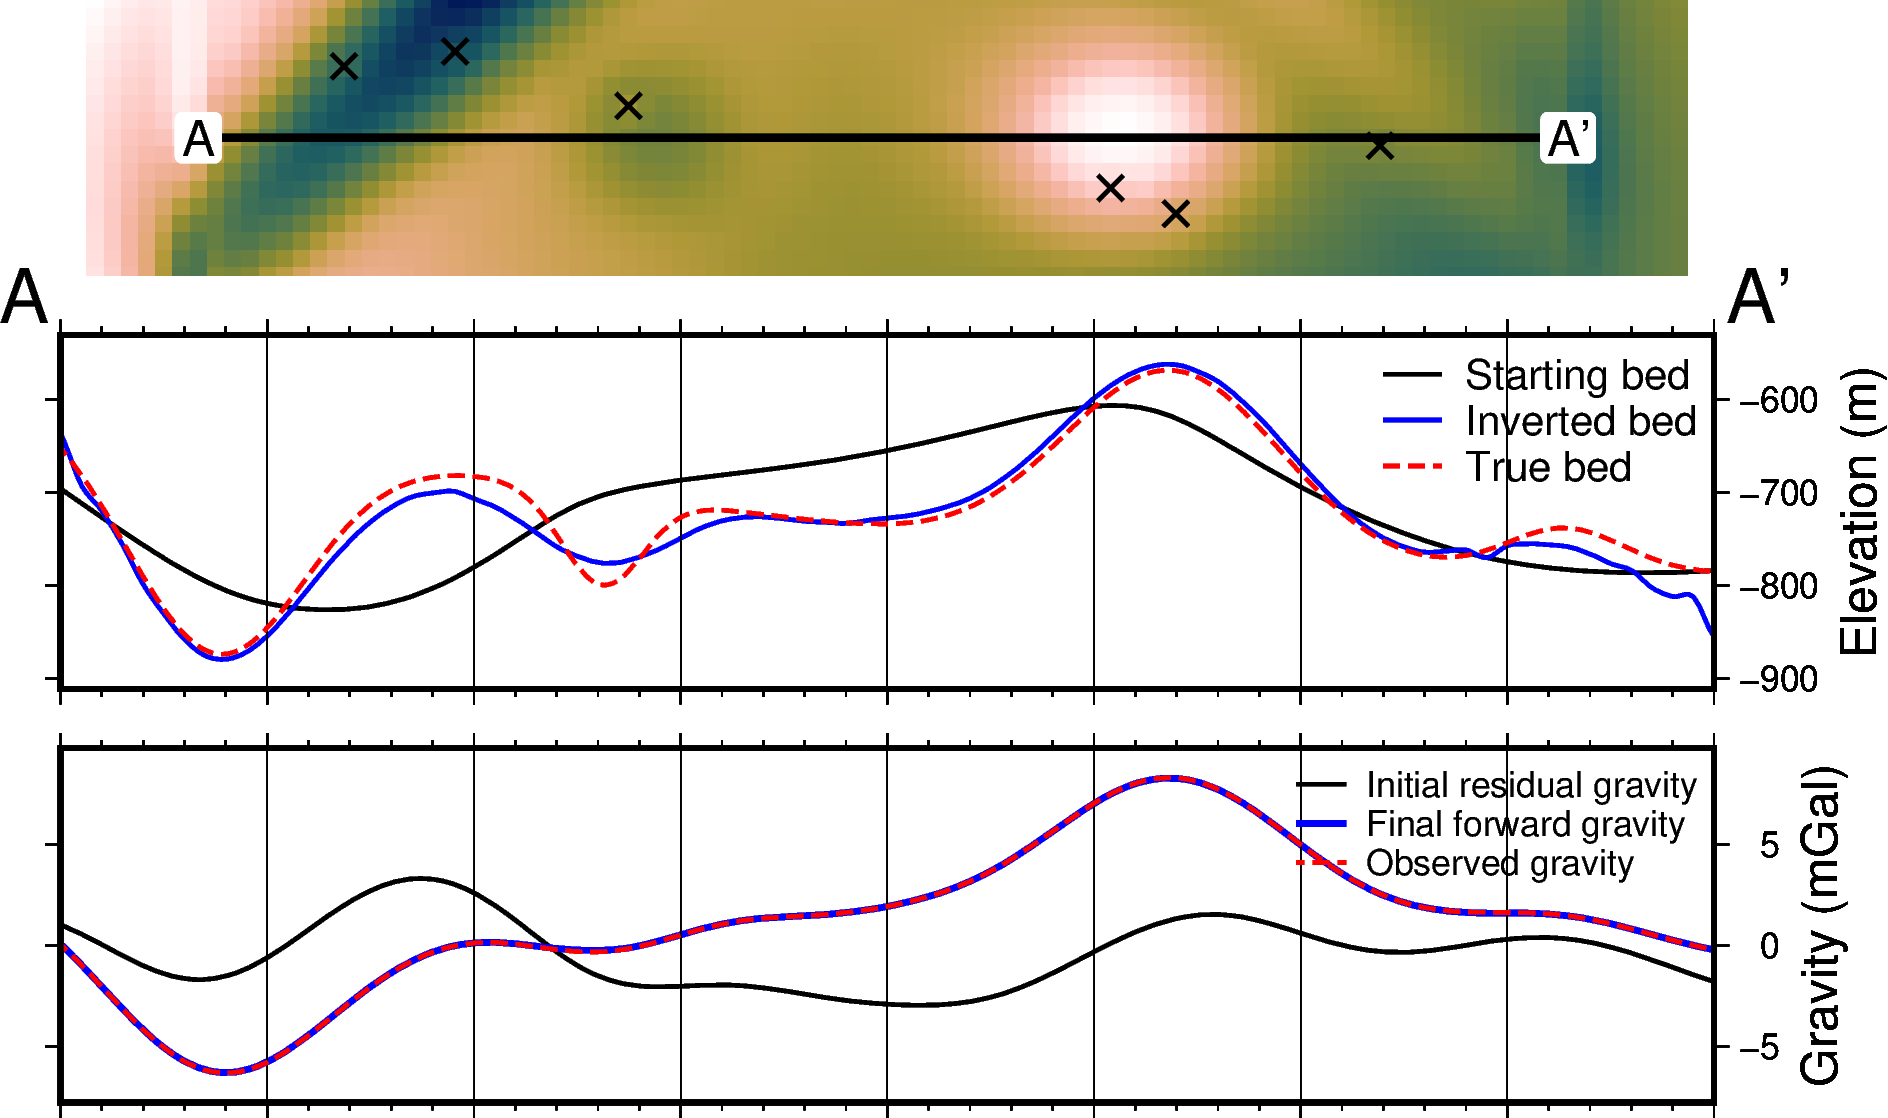
\includegraphics[width=\textwidth]{figures/chp3/chp3_simple_regional_sampled_profile.png}
        \caption{}
    \end{subfigure}
  \caption[Synthetic inversion with regional and re-sampling, CV and profile]{Cross-validation and profiles for the simple synthetic inversion with a regional component removed and low-resolution gravity data. a) Cross-validation curve showing the optimal damping parameter (red square). b) 2D profile of the inversion results. The top panel shows profile location and constraint points (black crosses). The middle panel contains topographic profiles of the starting, inverted, and true bathymetries. The bottom panel contains gravity anomaly profiles.}
    \label{fig:appB_simple_regional_sampled_CV_and_profile}
\end{figure}

\begin{figure}[!ht]
    \centering
    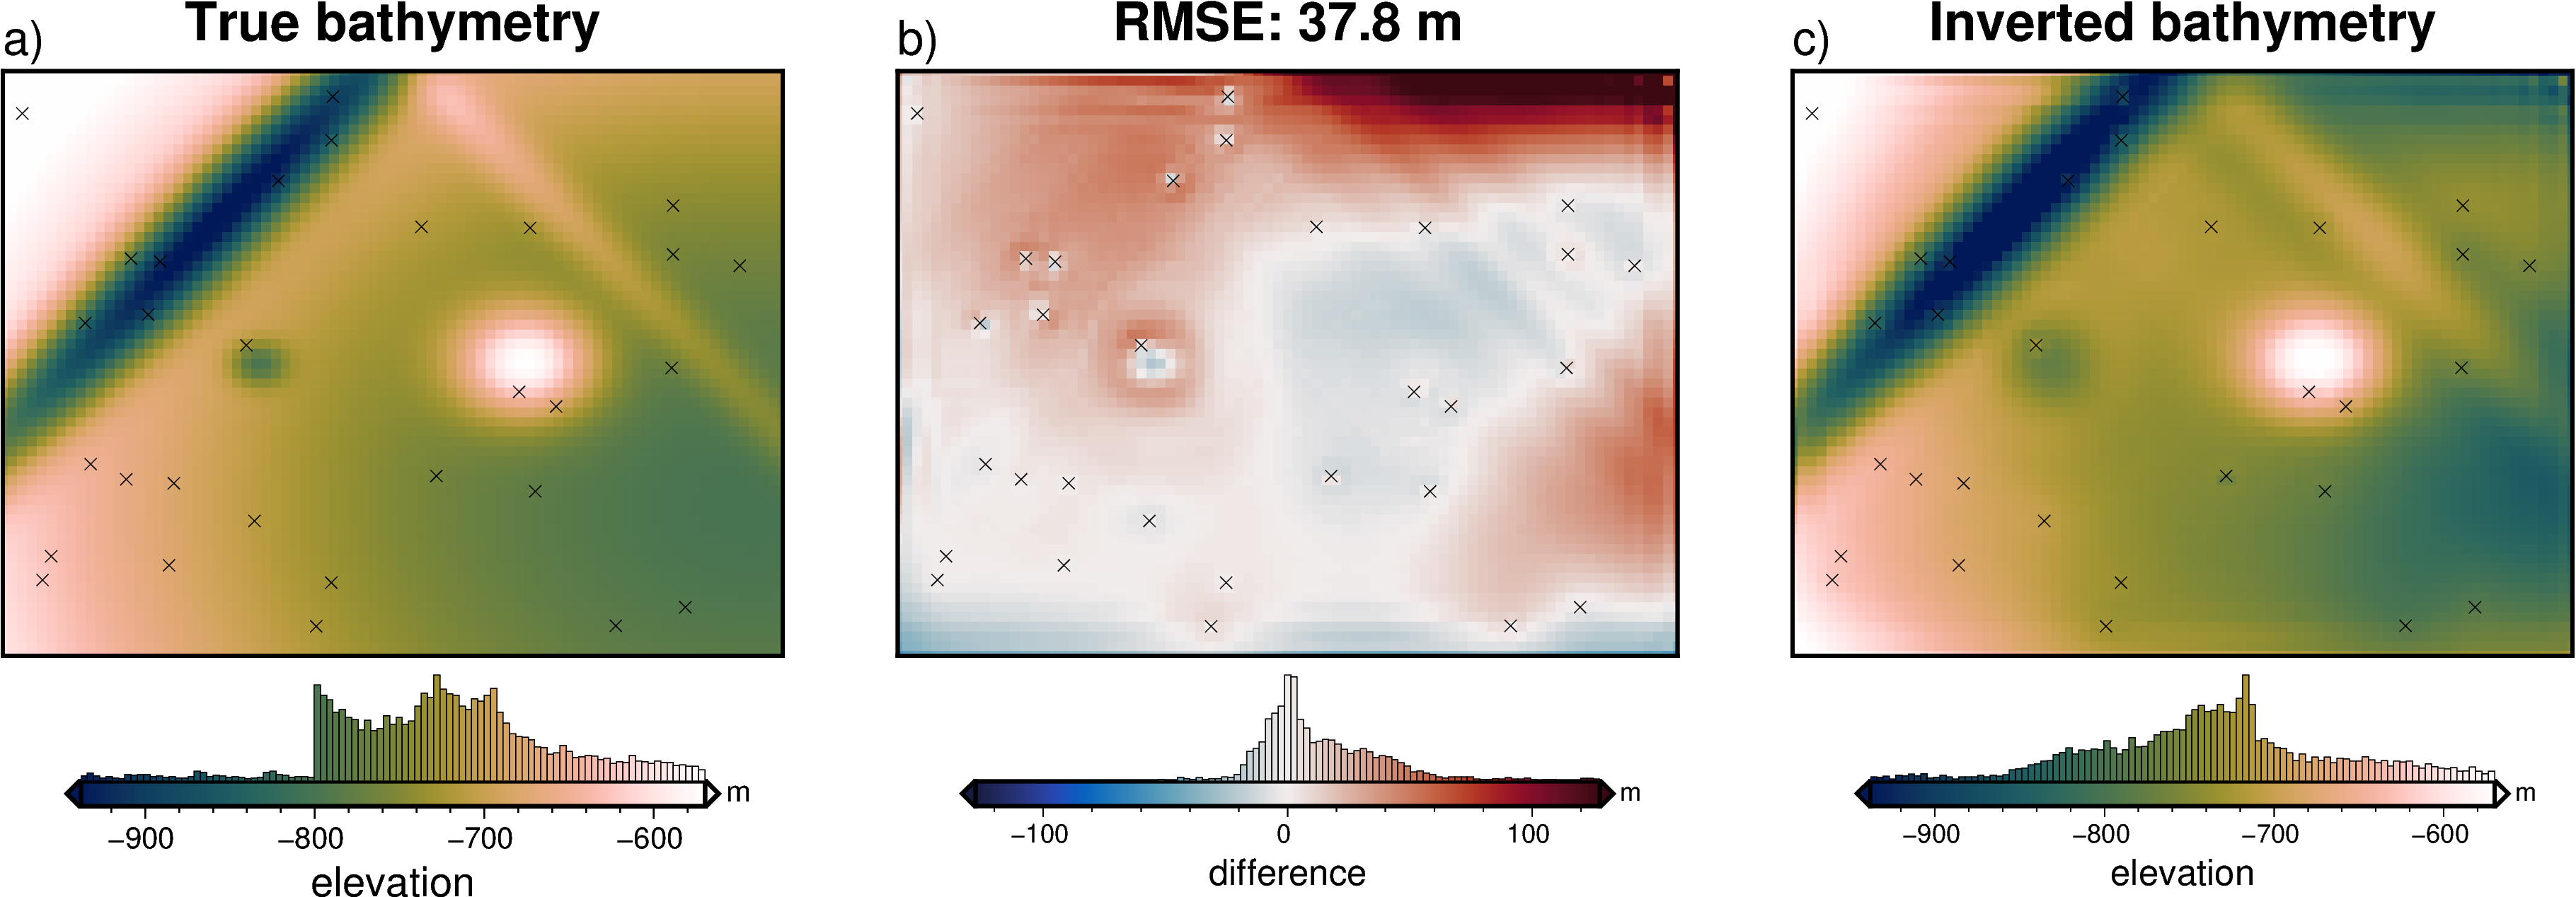
\includegraphics[width=.95\textwidth]{figures/chp3/chp3_simple_regional_sampled_results.png}
    \caption[Synthetic inversion with regional and re-sampling, results]{Simple synthetic model inversion with a removed regional component and gravity re-sampling. a) True bathymetry, b) difference between a) and c), c) final inverted bathymetry. Black crosses are constraint points. The RMS difference with the true bathymetry at these constraints is 2 m.}
    \label{fig:appB_simple_regional_sampled_results}
\end{figure}

\begin{figure}[!ht]
    \centering
    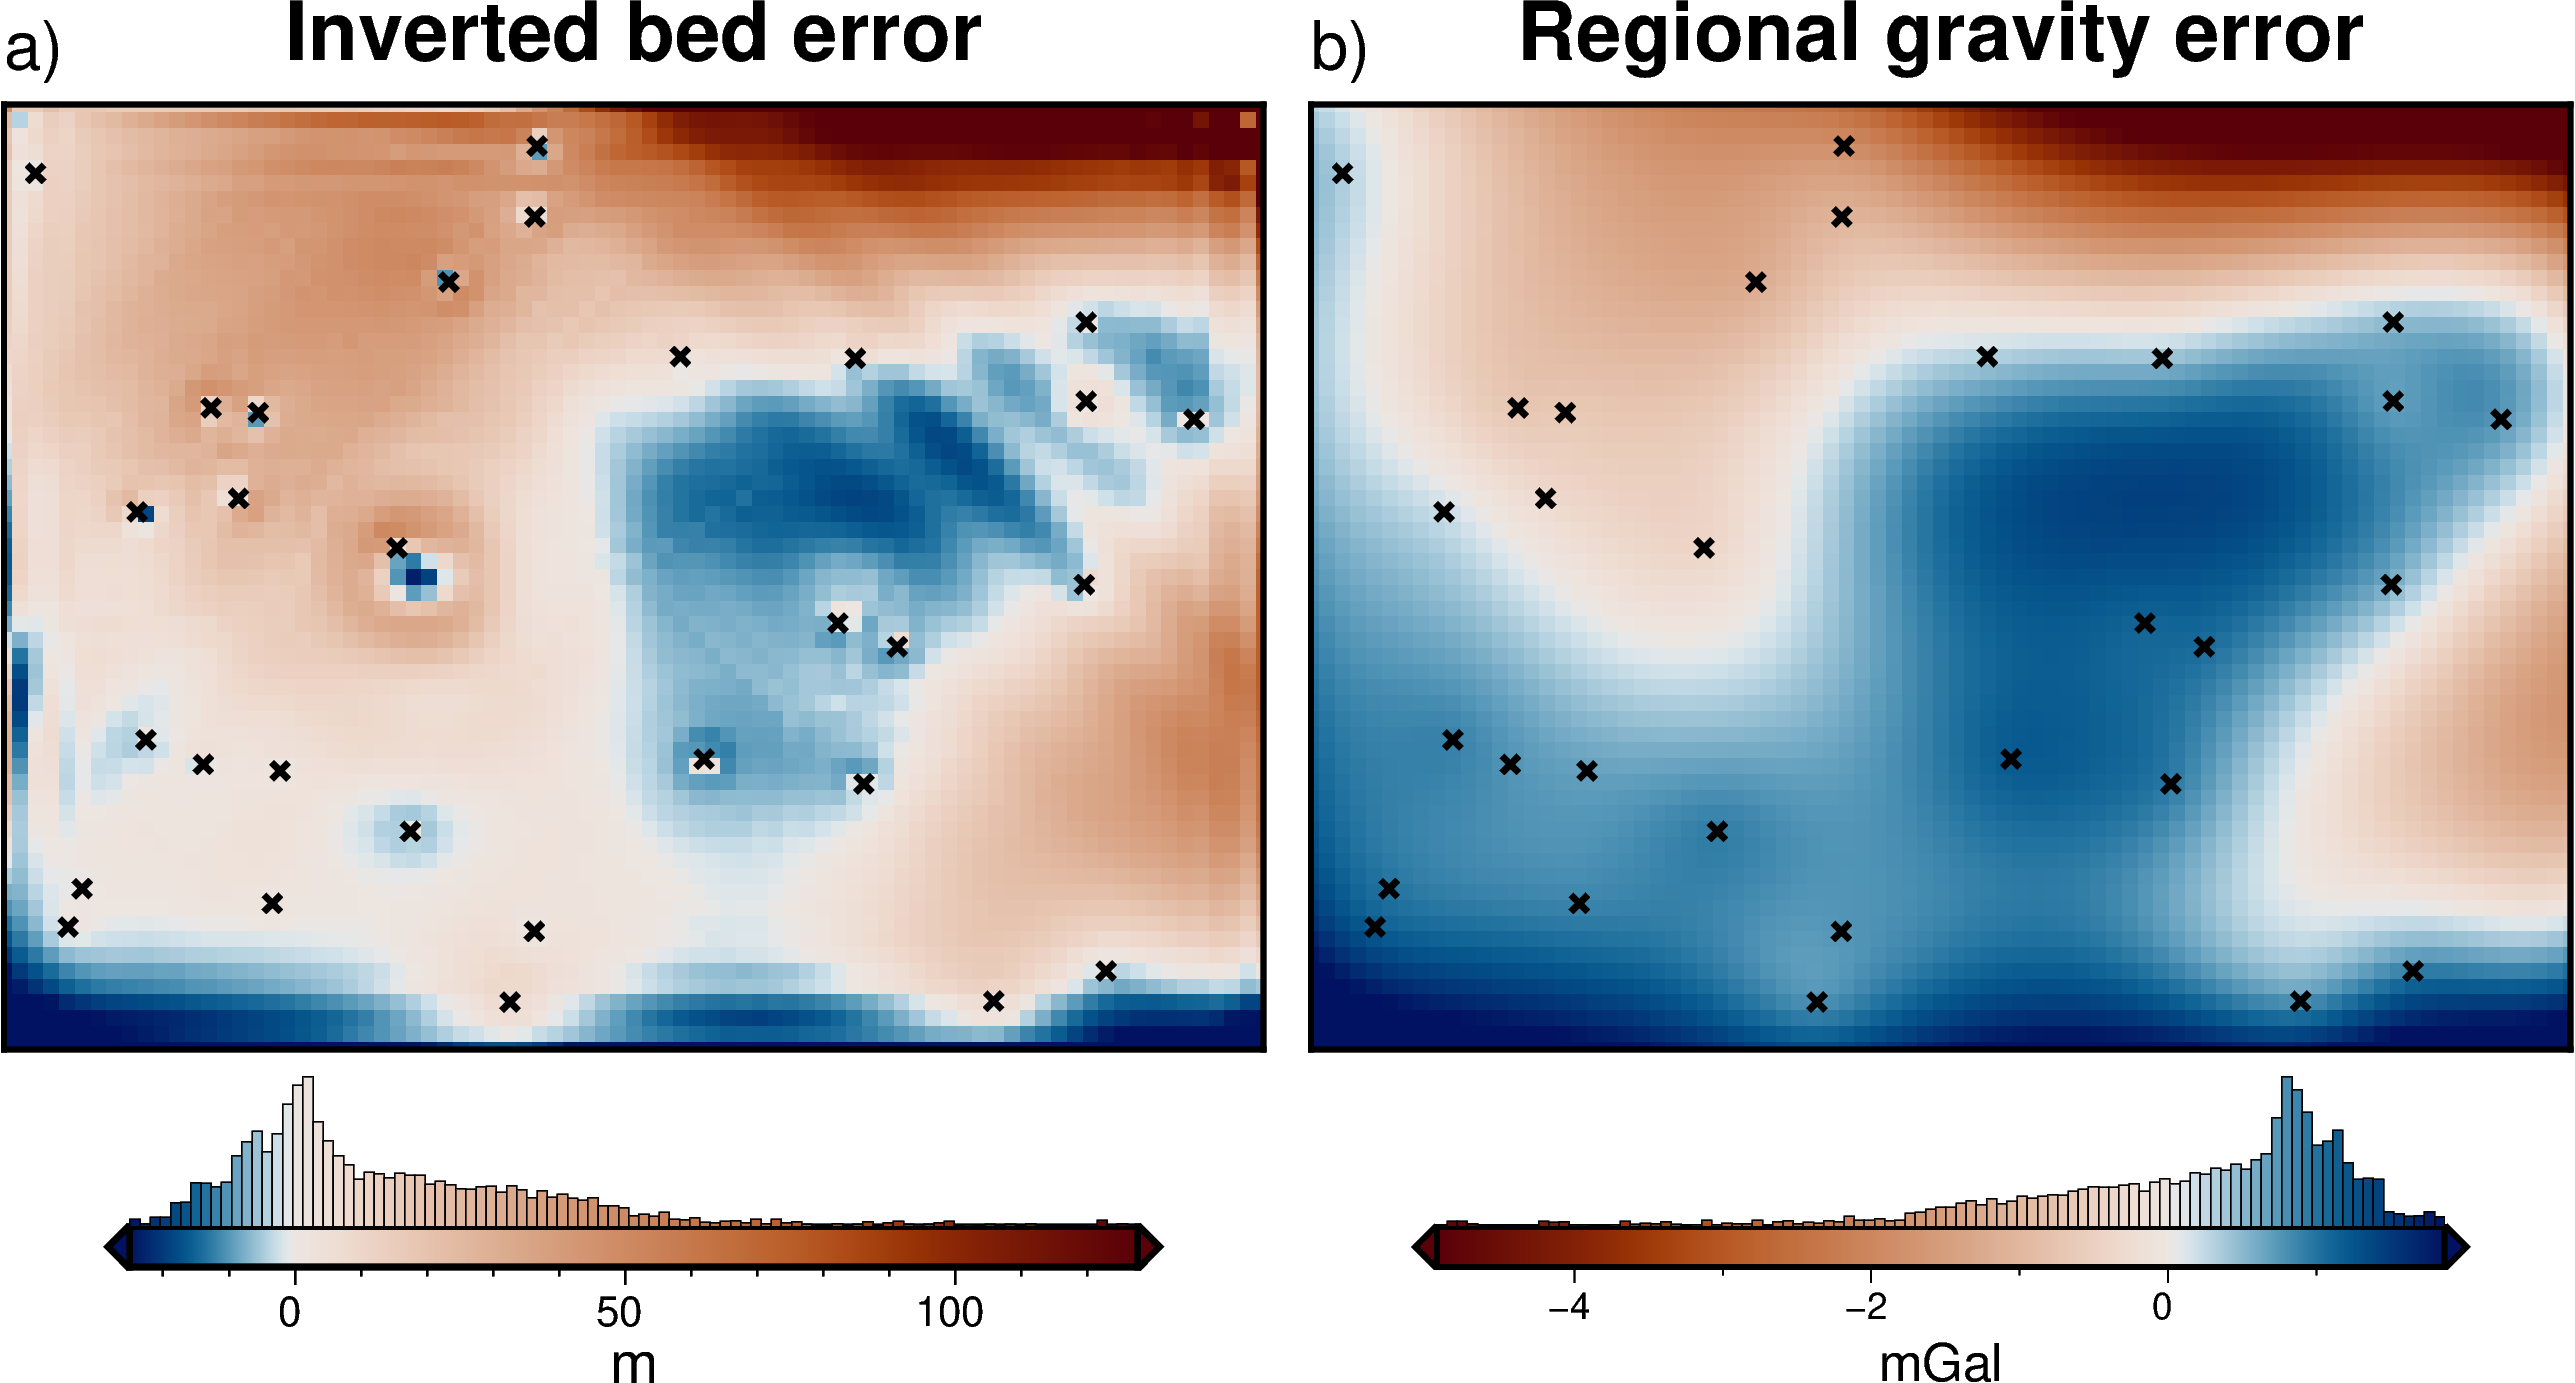
\includegraphics[width=.7\textwidth]{figures/chp3/chp3_simple_regional_sampled_bed_error.png}
    \caption[Inversion and regional error for model with regional and low-res gravity]{Source of inverted bathymetry error for model with regional field and re-sampled gravity data. a) Inverted bathymetry error from Figure \ref{fig:chp3_simple_regional_results}b. b) Error in the estimation of the regional component of gravity from comparison with the true regional component (Figure \ref{fig:chp3_simple_regional_gravity}b). Black crosses show constraint points. Colourmaps are opposed to highlight the similarities and the mean has been removed from the regional error.}
    \label{fig:appB_simple_regional_sampled_bed_error}
\end{figure}


\section{Ross Sea synthetic model}\label{appB_Ross_Sea}

\begin{figure}[!ht]
    \centering
    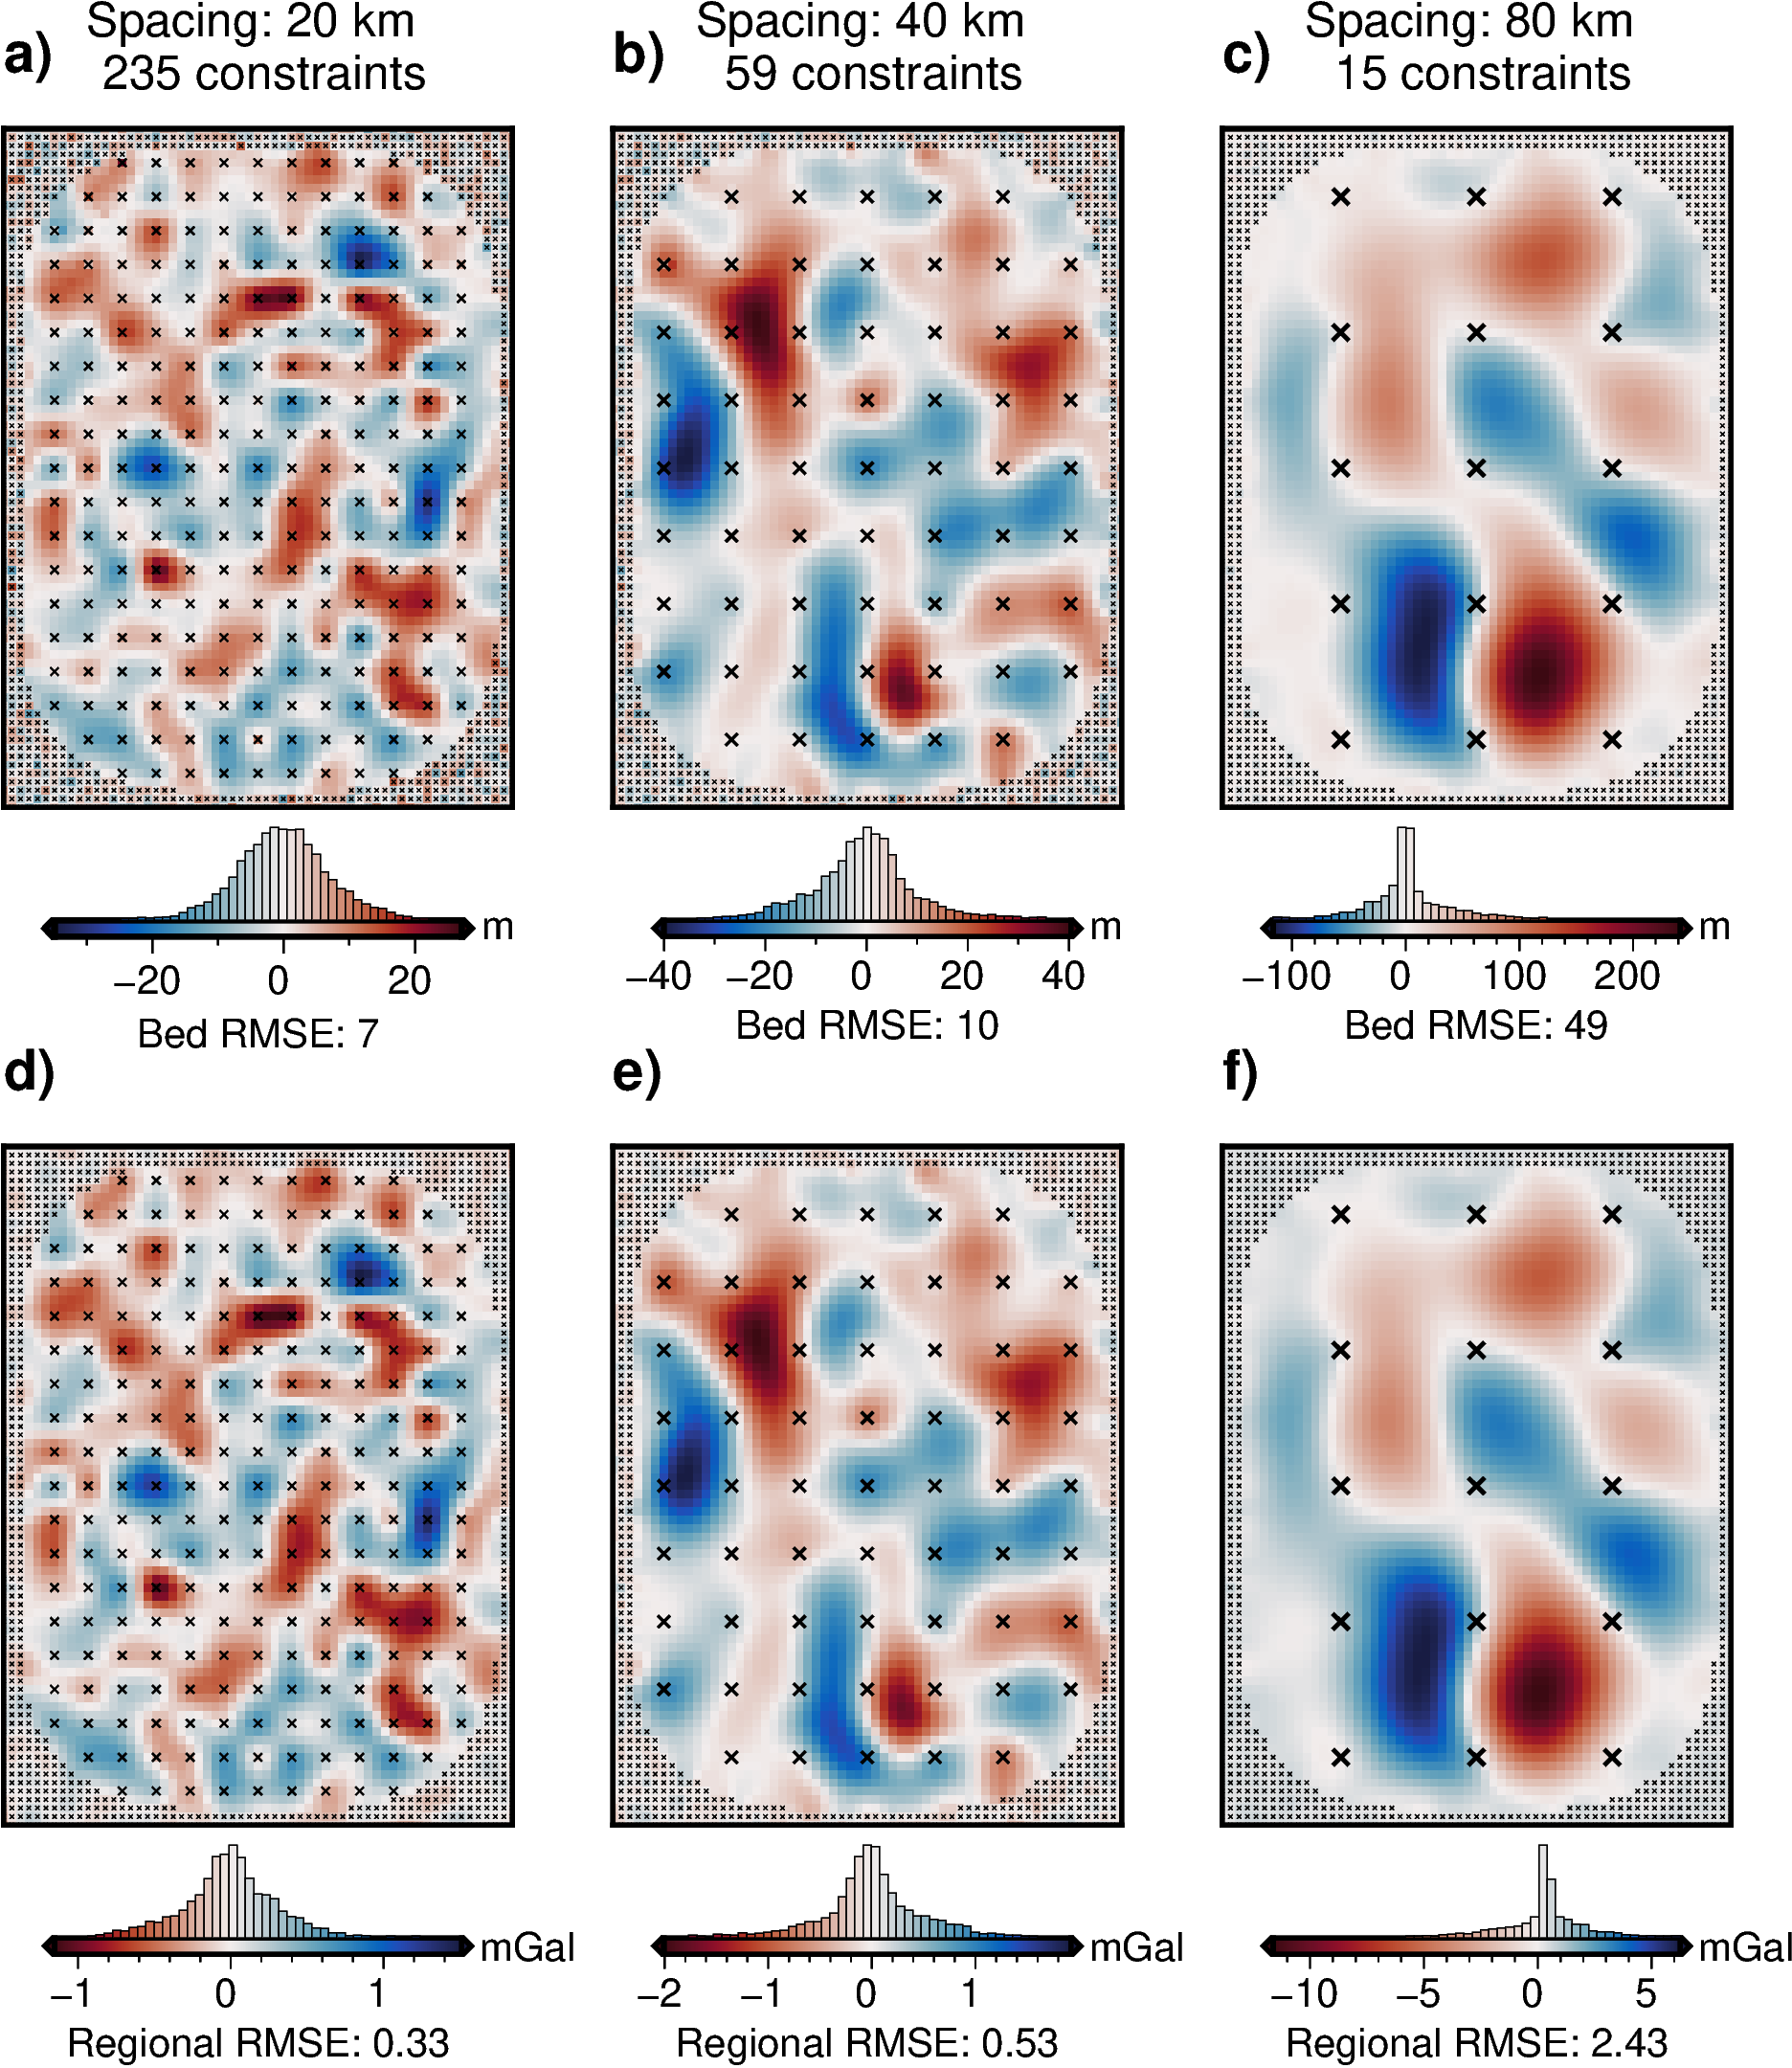
\includegraphics[width=.7\textwidth]{figures/chp3/chp3_Ross_Sea_constraints_ensemble_bed_regional_errors.png}
    \caption[Inversion and regional error for Ross Sea constraint ensemble]{Source of inverted bathymetry error for three inversion with varying constraint spacings. a) Inverted bathymetry error from three of the models in the constraint ensemble of Figure \ref{fig:chp3_Ross_Sea_constraints_ensemble}. b) Error in the estimation of the regional component of gravity from comparison with the true regional component for each model. Black crosses show constraint points. Colourmaps are opposed to highlight the similarities and the mean has been removed from the regional error.}
    \label{fig:appB_Ross_Sea_constraint_ensemble_bed_error}
\end{figure}

% \section{Computation times} \label{appB_comp_times}

% Analysis in this study was executed on a computer with an x86\_64 processor with a maximum clock frequency of 2600 MHz with 56 physical cores, 112 logical cores, and 1TB of RAM, using the Operating System Linux-Ubuntu. 

% The computation times reported through the text, both execution time and response time \citep{harris-birtillunderstanding2021}, were measured for various portions of this study, and are shown in Table \ref{table:ch3_comp_times}.

% \begin{tabular}{ |p{.4\textwidth}||p{.3\textwidth}|p{.15\textwidth}|p{.15\textwidth}|  }
%  \hline
%  \multicolumn{4}{|c|}{Computation times} \\
%  \hline
%  Chapter section & \# iterations & Execution time (hr:min:sec) & Response time (hr:min:sec) \\
%  \hline
% \ref{chp3:simple_model} Dual parameter Cross-Validation & 40 & 00:16:42  & N/A \\
% \ref{chp3:simple_model} Inversion & 43 & 00:01:01 & N/A \\
% \ref{chp3:simple_model} Damping Optimization with noise & 16 & -- & -- \\
% \ref{chp3:simple_model} Inversion with noise & 7 & 00:00:06 & N/A \\
% \ref{chp3:simple_model} Damping Optimization with sampled gravity & 16 & 00:01:04 & -- \\
% \ref{chp3:simple_ensemble}Noise and cell size ensemble & 100 & 08:48:05 & -- \\
% \ref{chp3:simple_regional_ensemble}Noise and cell size ensemble & 100 & 07:00:00 & -- \\
% \ref{chp3:Ross_Sea} Forward calculation of true model & $2.08e10^{5}$ prisms $\times$ $5.4e^{5}$ observations = $1.12e^{11}$ & 00:10:31 & -- \\
% \ref{chp3:Ross_Sea} Forward calculation of true model & $1.6e10^{4}$ prisms $\times$ $2.2e^{4}$ observations $\approx$ $3.5e^{8}$ & 00:00:03 & -- \\
% \ref{chp3:Ross_Sea} Equivalent source gridding of airborne survey & 9 parameter combinations & 00:01:07 & -- \\
%  \hline
% \label{table:ch3_comp_times}
% \caption{Ross Sea }
% \end{tabular}

\clearpage





\chapter{} \label{appendix:C}

This appendix provides supplemental information to Chapter \ref{ch:4}. 

\section{Gravity disturbance vs anomaly}

\begin{figure}[!ht]
    \centering
    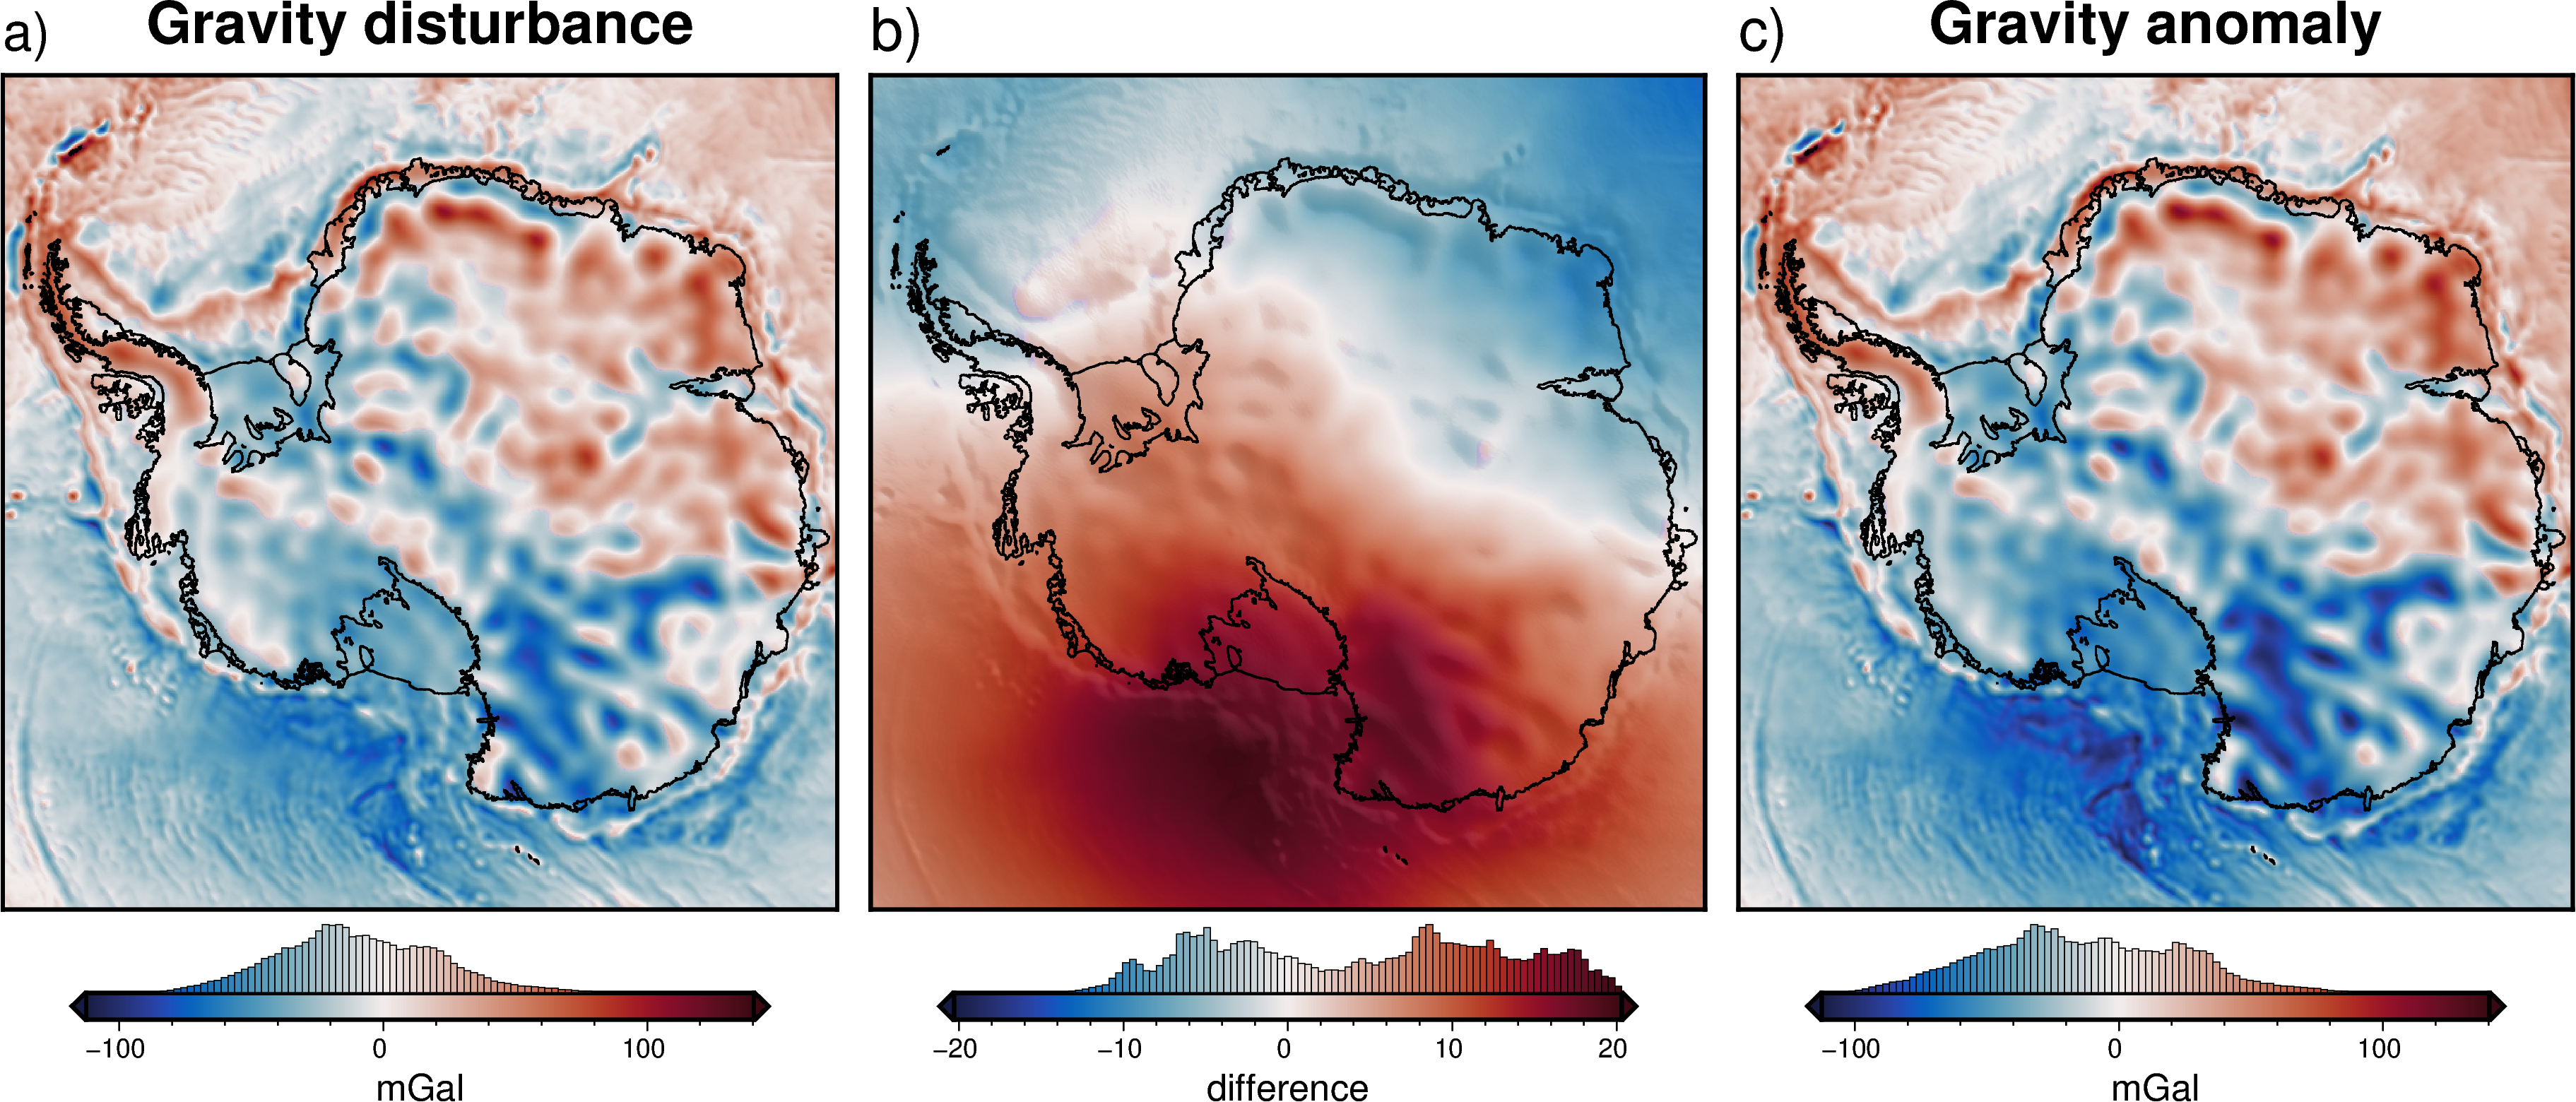
\includegraphics[width=.7\textwidth]{figures/chp4/antarctic_disturbance_vs_anomaly}
    \caption[Gravity disturbance vs. anomaly]{Difference between the gravity disturbance and anomaly for Antarctica. Observed gravity is from \citet{försteeigen6c42014} and the normal gravity for each was calculated with the python package Boule \citep{fatiandoaterraprojectboule2022}. See Section \ref{chp4:gravity_reduction} for further details.}
    \label{fig:appC_disturbance_vs_anomaly}
\end{figure}

\clearpage






\chapter{Antarctic-Plots} \label{appendix:D}

This appendix briefly describes the Python package Antarctic-Plots \citep{tankersleyantarctic2023} which I developed during this thesis and is used in all of the chapters. The documentation of the package is hosted at the following link; \url{https://antarctic-plots.readthedocs.io/en/latest/index.html} and the code is stored and developed in the following GitHub repository;  \url{https://github.com/mdtanker/antarctic_plots}. \\

The Antarctic-Plots Python package aims to help automate common tasks associated with researching Antarctica. There are four main modules of the package; \textbf{Fetch}, \textbf{Map}, \textbf{Profile}, and \textbf{Regions}.

\section{Fetch}

The Fetch module contains functions to download data related to Antarctica. These downloads are accomplished with the Python package Pooch \citet{uiedapooch2020}. Calls to these functions will download the respective data and store it in a common folder in your system. Subsequent calls to the same function will retrieve the already downloaded file. There is no need for remembering file paths or having multiple copies of the same data throughout your projects. Additionally, some of this data is pre-processed. This pre-processing includes re-projecting all data (gridded or tabular) to a common projection, South Polar Stereographic (EPSG:3031), and converting pre-gridded tabular data into more useful formats, such as Xarray dataarrays. \citep{hoyerxarray2017}.

This module currently contains over 40 datasets, which include; topography products, imagery, grounding line, coastline, and basin shapefiles, gravity, magnetics, geothermal heat flow, ice velocity, sediment thickness, moho depths, basal melt, ice mass change, and geologic units and faults. Below is an example that downloads, or retrieves if already download, BedMachine v3 surface elevation data, converted to be referenced to the WGS-84 ellipsoid (as opposed to the original data which is referenced to the geoid), and resampled at a 5 km spacing.
\begin{python}
from antarctic_plots import fetch

surface_data = fetch.bedmachine(
    layer="surface", 
    reference="ellipsoid", 
    spacing=5000,
)
\end{python}

\section{Map}

The Map module provides convenient methods for plotting geospatial data. Most of these plotting functions use the Python package PyGMT \citep{uiedapygmt2021}. All of the maps in Chapters \ref{ch:3}, \ref{ch:4}, \& \ref{ch:5} were created with the help of these functions. In addition to static figures, there are several functions for creating interactive figures, which help with data visualization. 

\section{Profile}

The Profile module is used to sample gridded data along specified profiles, and plot cross-sections and profiles of the data. The cross-section plots of Chapters \ref{ch:3} \& \ref{ch:4} were created using these functions. Profiles can be defined by clicking on an interactive map to help with quickly exploring and visualizing datasets. 

\section{Regions}

The Regions module provides pre-defined variables of region boundaries in EPSG:3031 for commonly studied Antarctic areas. These region variables are used by the other modules to subset the desired region. For example, if you only want to fetch BedMap2 surface topography only for the Ross Ice Shelf, instead of the whole continent, you can pass the parameter "region = regions.ross\_ice\_shelf".

Additionally, there are geospatial tools provided for re-projecting, masking, and gridding data. This package is still early in its development and many more datasets and functions will still be added. 